% Built by scripts/08_draft_to_tex.R from docs/draft/draft_v3.md. Edit the Markdown, then rerun the script.
% Compile from docs/draft: pdflatex draft_v3.tex (twice). Tables are \input from results/tables/paper; figures from results/figures/paper.
% Table numbering in this file is sequential; the Markdown labels tables by section (e.g. Table 6a). The bracketed file names in the text identify each table.
\documentclass[11pt]{article}
\usepackage[margin=1in]{geometry}
\usepackage{amsmath,amssymb}
\usepackage{booktabs,threeparttable,graphicx,float,longtable,array}
\usepackage{hanging}
\usepackage[hidelinks]{hyperref}
\usepackage{xurl}
\emergencystretch 3em
\usepackage{setspace}\onehalfspacing
\usepackage[T1]{fontenc}\usepackage[utf8]{inputenc}\usepackage{lmodern}
\setcounter{secnumdepth}{1}
\title{A Bright Line That Binds on Few: The NBA's 65-Game Rule and Star Availability}
\author{Luke Maddock\\ \small Department of Data Analytics, Denison University}
\date{Draft v3.1, 2026-09-16. Every number is taken from a saved table. Bracketed citations name files in \texttt{results/tables/paper/} unless a longer path is given; figures are in \texttt{results/figures/paper/}.}
\begin{document}
\maketitle



\begin{abstract}
In 2023-24 the NBA made eligibility for its major individual awards conditional on appearing in 65 regular-season games of at least 20 minutes. The rule is a notch, and notches predict bunching at the threshold, play-through by players just short of it, and more rest once eligibility is secured or out of reach. Using every player-game from 2013-14 through 2025-26, I test each prediction against the players who meet the league's own definition of a star and find no mark on games played. There is no excess mass at 65. Stars near the line late in the season were no more likely to cross it. Star availability relative to comparable players defined on prior-season status changed by -0.8 games (SE 2.3) after the rule, with a minimum detectable effect of 6.5 games, and the raw rise in star games in the rule's first season was half a change in who the stars were and half a within-player swing of a size seen before the rule. Late-season absence by stars who had played the previous game shows the same injury-driven gradient across eligibility states before and after the rule. The explanation is arithmetic: only a quarter of stars are within reach of the line in the season's last weeks, and a full response by all of them would add at most 0.7 to 1.3 games to the star mean. The one detectable effect is on minutes. The share of star appearances lasting 20 or more minutes rose 4.6 percentage points (SE 1.0) relative to the control group, which did not move. I also document that ESPN box scores omit players on the inactive list, so absence must be measured on the schedule rather than on box-score rows.
\end{abstract}

\noindent \emph{JEL codes:} J22, J33, Z22, H24, D91.\\ \emph{Keywords:} notches, bunching, awards, tournaments, labor supply, load management, National Basketball Association.

\clearpage


\section{Introduction}


In April 2024 the NBA commissioner reported that games missed by star players had fallen about 15 percent in the first season of the league's 65-game award-eligibility rule (Sportico 2024). The raw numbers agree: stars averaged 59.4 games in 2022-23 and 65.0 in 2023-24 {\small\texttt{[tab1\_sample]}}. Half of that rise was a change in who the stars were. The seven players who entered the star set in 2023-24 averaged 69.6 games and the six who left had averaged 46.7 the season before. The 39 players who were stars in both seasons played 2.9 more games, a within-player rise of a size the same comparison had produced from 2015 to 2016 and would produce, in the other direction, from 2025 to 2026 {\small\texttt{[tabA8\_composition\_2024; tabA9\_cohort\_pairs]}}. This paper asks whether the rule changed star behavior at all, and answers with bounds.

The rule is a notch in the sense of Kleven and Waseem (2013). To be eligible for Most Valuable Player, Defensive Player of the Year, and the All-NBA and All-Defensive teams, a player must appear in 65 regular-season games of at least 20 minutes, with an allowance of two games between 15 and 19 minutes. Below the line the award system offers nothing; at the line it offers full eligibility. Notches predict mass at the threshold, play-through by agents just short of it, and slack once eligibility is either secured or out of reach. The direction of these predictions does not depend on the size of the prize; the magnitude does, which is why Section 7 counts the players for whom the prize is large and pivotal. Where that population is thin, the bunching literature has long recognized that no visible response should be expected (Saez 2010; Chetty et al. 2011; Kleven 2016).

I test each prediction on every player-game from 2013-14 through 2025-26, for the 36 to 46 players per season who meet the league's own definition of a star. There is no excess mass at 65. Stars within a few games of the line late in the season were no more likely to cross it after the rule than before. Star availability relative to a control group defined on prior-season status did not change in any post-rule season; the pooled estimate for games played is -0.8 (SE 2.3) with a minimum detectable effect of 6.5 games. Late-season absence among stars who had played the previous game did not rise in the states where the rule removes the incentive to play. The reason is that the rule can matter only to the quarter of stars within reach of the line in the season's final weeks, and a complete response by all of them would add between 0.7 and 1.3 games to the star mean, inside every interval reported. Star absence is dominated by spells of ten or more games, which the rule does not touch. The one detectable effect is on minutes: after the rule, stars almost never appear for fewer than 20 minutes, and the share of their appearances that qualify rose 4.6 points (SE 1.0) relative to the control, which did not move.

The paper makes three contributions. To my knowledge it is the first econometric evaluation of the rule or of the Player Participation Policy (PPP) adopted alongside it; the nearest academic work studies the performance effects of rest by age and cites the policy only as motivation (Nakamura-Sakai, Forastiere, and Macdonald 2024). To the literature on notches it adds a case in which a clean notch with real stakes produced no detectable response on the targeted margin and a detectable response on an adjacent one, and it traces the null to the size of the population at the margin rather than to a zero elasticity. And it documents, for users of ESPN box scores, that the source carries only players on the active list, so that absence must be measured on the schedule.

Section 2 reviews the rule, the policies around it, and the literatures the paper draws on. Section 3 sets out a simple model. Section 4 describes the data. Sections 5 and 6 report availability and absence results. Section 7 formalizes the mechanisms and reports the minutes effect. Section 8 discusses what the results do and do not show.


\section{Background}



\subsection*{The rule and the policies around it}


Figure 1 places the policies on a timeline. The 65-game rule was ratified in the April 2023 collective bargaining agreement and applied from 2023-24. A game counts if the player plays at least 20 minutes; up to two games of 15 to 19 minutes also count. Rookie of the Year is exempt (ESPN 2023b). The in-season tournament final counts toward the threshold although it is excluded from regular-season statistics (Sports Illustrated 2026). There is an exception for season-ending injuries after 62 qualifying games and a provision for extraordinary circumstances. In April 2026 the league and the union ruled two players eligible under that provision, one at 64 qualifying games who missed two games for the birth of a child and one at 63 after a collapsed lung, while a third, at 60, took his case to an arbitrator and lost (ESPN 2026; Forbes 2026). My counts for those three players are 64, 63, and 60 {\small\texttt{[waiver\_cases\_2026.csv]}}. A fourth player reached 65 in the season's penultimate game by playing 26 minutes through bruised ribs, his 64 regular-season games plus the tournament final (FOX Sports 2026); my count is 64 regular-season games and 65 under the rule {\small\texttt{[tabA5\_bbr\_validation]}}.

The stakes are large for a minority. All-NBA selection triggers salary escalators and eligibility for the largest contract tiers, and one player's exclusion from the 2023 teams was reported to cost him 39 million dollars over five seasons (Sportico 2023). For the median star the stakes are smaller: an All-NBA third team is a distinction, and Sixth Man or Most Improved is not a target for a player already recognized as a star.

The rule was written against a specific fact: in 2023, five of the fifteen All-NBA selections had played fewer than 65 games (Hoops Rumors 2024a). The PPP took effect in the same season. It defines a star as a player selected to an All-Star or All-NBA team in any of the prior three seasons, requires teams to keep healthy stars available for nationally televised and tournament games, forbids resting two stars in one game, requires a balance of home and road absences, bars long shutdowns of healthy players, and fines teams 100,000 dollars for a first violation, 250,000 for a second, and one million more than the previous penalty thereafter (NBA 2023; ESPN 2023a). A resting policy adopted in September 2017 already barred resting healthy players on national television and resting several players at once, and the league restated it twice before the PPP. A November 2019 memo barred teams from labeling a healthy player's absence `\texttt{load management,'' reserving }`rest'' for that case and reminding teams that healthy players could not sit high-profile televised games; the Clippers were fined 50,000 dollars that month over statements about Kawhi Leonard's health that the league found inconsistent with his status (ESPN 2019; CBS Sports 2019). A December 2020 memo for the condensed pandemic season reaffirmed the television-game prohibition, with a fine of at least 100,000 dollars, while allowing rest in non-televised games for back-to-backs, veterans coming off a long playoff run, and players recovering from COVID-19 (ESPN 2020; NBC Sports 2020). The PPP's additions in 2023 were the star definition, the escalating fines, the roster-balance and no-shutdown provisions, and enforcement (ESPN 2023b). The PPP acts on the team, not the player.


\subsection*{Notches, bunching, and thresholds in sport}


Saez (2010) compared the density of taxable income around kink points with a smooth counterfactual and recovered elasticities from the excess mass; his headline result is a set of nulls, with clear bunching at one kink only and only among the self-employed. Chetty et al. (2011) showed that optimization frictions attenuate bunching and that kinks affecting larger groups produce larger observed responses. Kleven and Waseem (2013) extended the method to notches and showed that large shares of agents remain in dominated regions, which identifies frictions. Kleven (2016) states the caveat that governs this paper: absence of bunching implies either a low structural elasticity or high frictions, and the data around the threshold cannot separate them. Bertanha, McCallum, and Seegert (2023) provide inference for the partially identified case, which is the frame for the bounds reported here.

Thresholds in sport have produced some of the clearest bunching evidence outside tax data. Pope and Simonsohn (2011) show that batters entering a season's final at-bat at .298 or .299 hit .463 in it, and Allen et al. (2017) find marathon times piling up just under round numbers. Both settings share features the 65-game rule lacks: the threshold sits near the center of the outcome distribution and the marginal action is cheap and available to everyone near the line. A games threshold sits in the upper tail of a distribution shaped mostly by injury, and the marginal action is unavailable to an injured player.


\subsection*{Awards and tournaments as incentives}


The rule conditions access to a rank-order tournament. Lazear and Rosen (1981) showed that effort responds to the spread between prizes, and Ehrenberg and Bognanno (1990) confirmed it on the golf tour. Awards without money attached also move behavior: Kosfeld and Neckermann (2011) found that symbolic awards raised performance in a field experiment, Neckermann, Cueni, and Frey (2014) found the same for workplace awards, and Chan et al. (2014) for academic honors; Frey and Gallus (2017) treat awards as a distinct instrument. These results justify treating All-NBA selection as an incentive even where no bonus is written into a contract, and they make the null more informative: the prize is one people respond to.


\subsection*{Strategic responses in sports labor markets}


Kahn (2000) made the case for sports data as a labor-market laboratory. NBA players respond to individual financial incentives at some margins and not others: Stiroh (2007) found performance rising before a new contract and falling after, and Owsik and Tan (2026) find no regular-season contract-year effect but a decline after signing. Teams respond to bright-line league rules: Taylor and Trogdon (2002) and Price et al. (2010) show teams losing more often when the draft rewards losing, Fumarco et al. (2024) document responses to contractual thresholds in hockey, and a 2024 case in which a baseball player was released four plate appearances short of a bonus is the mirror image of the individual incentive studied here (CBS Sports 2024). The 65-game rule differs from these settings in that the threshold applies to a named class of players and interacts with an injury process the player does not control.


\subsection*{Why star availability matters, and what drives it}


Rosen (1981) explained why a few performers capture a disproportionate share of a market's value. Hausman and Leonard (1997) put the value of one star to the other teams in the league at about 53 million dollars, and Kaplan (2022) found that a superstar's announced absence lowers secondary-market ticket prices by 4 to 22 percent, more for road games; Kaplan et al. (2019) is the conference precursor. That externality is what the PPP is designed to internalize. On the supply side, Teramoto et al. (2017) tied game injuries to back-to-back and road games, with the caution of Mack et al. (2018) that exposures are not risks; Esteves et al. (2021) show that schedule congestion degrades performance; and Torres-Ronda et al. (2022) count more than 800 injuries per season, concentrated in the middle and late season. League figures for 2024-25 reported games missed to injury up 13 percent and stars missing 19 percent of games to injury in each post-rule season, the same as in 2017-18 and 2018-19 (Sportico 2025). These are press figures, but they set the scale: injury absence is an order of magnitude larger than anything a rest policy could reach.


\subsection*{Competing work}


A search of SSRN, NBER, arXiv, the MIT Sloan Sports Analytics Conference, and Google Scholar returned no article, working paper, or thesis that evaluates the 65-game rule or the PPP as its research question. The nearest item is Nakamura-Sakai, Forastiere, and Macdonald (2024). The league's own claims about the rule's effect are descriptive (Sportico 2024). Section 5.2 shows what the raw comparison consists of.


\section{A simple model}


\begin{quote}
``I guess use your 17 games as wisely as possible.'' Bam Adebayo, January 2024, on the 65-game rule (Hoops Rumors 2024a).
\end{quote}


Consider a star deciding, game by game, whether to play. Let $q$ be the number of qualifying games so far, $r$ the number of games remaining, and $\bar q = 65$ the threshold. Each game played yields a flow benefit $b$ and carries a cost $c_g$ that varies with fatigue, minor injury, and schedule. Eligibility is worth $V \geq 0$ and is received if and only if $q \geq \bar q$ at season's end. Before the rule $V$ enters continuously through voters' impressions; after it, as a step.

Three predictions follow. A player who reaches exactly 65 has no further eligibility motive to play, so mass should collect at the threshold and thin just above it. Define slack as $q + r - \bar q$, the number of remaining games a player can miss and still reach the line. For players with small non-negative slack late in the season, the option value of eligibility raises the return to playing through a marginal cost, so the share reaching 65 should rise after the rule, most among players for whom $V$ is largest. Once slack is negative or $q \geq \bar q$, the marginal eligibility incentive is zero, so absence in those states should rise relative to the reachable state.

A fourth prediction concerns minutes. Because a game counts only at 20 minutes, a player or coach who wants a game to count will not let an appearance end at 18 minutes. After the rule, the share of star appearances lasting at least 20 minutes should rise, and rise most for players near the line. This margin is cheap in a way that games are not: it requires no additional appearance, only that an appearance already being made be long enough to count.

The magnitude of every prediction scales with $V$ and with the number of players for whom the threshold is pivotal. A player who would have played 75 games regardless is unaffected; so is a player whose injury ends the season at 40. Section 7 counts the pivotal population and bounds the aggregate effect. The PPP pushes against the third prediction: its fines apply in every state, so it predicts a uniform fall in discretionary absence.


\section{Data}



\subsection*{Sources and definitions}


Player-game box scores come from ESPN through hoopR (Gilani 2021), for regular seasons 2013-14 through 2025-26; seasons are indexed by end year. The 2019-20 and 2020-21 seasons are excluded from every estimate. Honors come from Basketball-Reference pages cached once, with the 2025 and 2026 All-Star rosters entered by hand. Estimation uses fixest (Bergé 2018).

A star in season $s$ is a player who made an All-Star or All-NBA team in any of seasons $s-3$ to $s-1$, the PPP's definition; because it is lagged it cannot respond to the treatment. There are 36 to 46 stars per season with at least one appearance {\small\texttt{[tab1\_sample]}}. A contender is a star who made an All-NBA team or received an MVP or Defensive Player of the Year vote in the prior season. The control group is defined the same way, on prior-season status: players who are not stars in season $s$ and who in season $s-1$ averaged at least 28 minutes per game and played at least 40 games. They number 68 to 90 per season from 2015 on; none can be defined for 2014. A robustness control uses rotation players, 20 or more minutes and 40 or more games in the prior season. Defining the control on the prior season matters. An earlier version of this analysis defined it on current-season minutes and games, which selects on the outcome: a control player could not have missed more than 42 games while a star could have missed 80, and the accompanying filter on rostered games truncated the stars' low tail. That design is retained as a labeled comparison row. Both controls are partially treated, since All-Defensive, Most Improved, and Sixth Man awards carry the same requirement.

Qualifying games follow the rule's definition and include the tournament final; games played is the regular-season statistic and excludes it. Slack, eligibility state, and the health condition are defined at the player-game level as in Section 3. The late-season window is team game 56 onward. A player is \emph{healthy} entering a game if he played his team's previous game.


\subsection*{What ESPN box scores contain}


An ESPN box score carries the players on a team's active list for that game: those who played, and those who dressed and did not play, who appear as a row with a reason string. Players on the inactive list, whether injured, ill, away from the team, or resting, do not appear at all. I verified this against seven Basketball-Reference box scores spanning 2015 to 2026, chosen so that a star had an absence with no ESPN row. All 40 ESPN did-not-play rows in those games appear inside the Basketball-Reference box as did-not-play or did-not-dress; none of the 51 players Basketball-Reference lists as inactive has an ESPN row; and all seven stars are on the inactive list {\small\texttt{[tabA14\_bbr\_boxscore\_check]}}.

The distinction matters because the two absence types have moved in opposite directions. Table 2 {\small\texttt{[tab2\_source\_coverage]}} reports the share of absences that appear as a dressed-but-unused row. For stars it was 28 to 40 percent in 2014 through 2017, 15 percent in 2018 and 2019, 7 to 10 percent in 2022 through 2024, and 8 to 16 percent after. For the control it fell from 30 to 38 percent in 2015-2017 to between 9 and 23 percent from 2022 on. The total absence rate of stars did not fall; it was between 14 and 32 percent of team-games in every season. Teams moved absent players from the bench to the inactive list. Any outcome computed from box-score rows therefore tracks roster designation, not behavior, and neither designation maps to rest versus injury. I build the player-game panel on the full schedule of each player's team stints, with a flag for whether a row exists.\footnote{The exploratory construction that counted only games with a row produced star ``rest'' rates of 7.1 percent in 2014 and 1.1 percent in 2023 [rest\_raw\_by\_season\_rowsonly.csv], a fall that coincides with the fall in row coverage in Table 2. Those replications are in Appendix Table A1.}


Two smaller corrections. ESPN files the All-Star and Rising Stars games as regular-season games; removing those rows lowers qualifying games by one for ten to seventeen stars per season through 2024, and three star-seasons cross 65 only because of them {\small\texttt{[tabA7\_exhibition\_correction]}}. And 14 flagged star-seasons outside the pandemic years have no appearance, mostly retired players still flagged from earlier honors {\small\texttt{[tabA6\_stars\_no\_appearance]}}. A check of ten star-seasons against Basketball-Reference finds all nine with a reference value matching exactly; the tenth played no games {\small\texttt{[tabA5\_bbr\_validation]}}.

The same source property limits what can be learned about rest. Among late-season absences by stars who had played the previous game, 45 percent had a dressed-but-unused row before the rule and 19 percent after. Of the reasons given, rest and coach's decision account for a quarter of all such absences before the rule and 2.6 percent after; the remainder are injury strings or inactive-list absences with no reason {\small\texttt{[tabA4\_absence\_reasons; rest\_absence\_reason\_bounds.csv]}}. Discretionary rest and new injury cannot be separated in this source.


\subsection*{The sample}


Table 1 {\small\texttt{[tab1\_sample]}} describes the sample. Stars averaged 59.4 games in 2023 and 65.0 in 2024; the share with at least 65 qualifying games went from 0.44 to 0.67. Both fell back in 2025 and 2026, to 62.4 and 54.8 games and to 0.54 and 0.47. The control averaged 65.6 games in 2023, 66.1 in 2024, 62.0 in 2025, and 58.8 in 2026.


\section{Availability results}



\subsection*{Event studies}


Figure 3 and Table 3a {\small\texttt{[tab3a\_availability\_event\_study]}} report event-study estimates of star availability relative to the control, with 2023 as the reference season, from a regression of games played or qualifying games on star-by-season indicators with player and season fixed effects, on all star and control player-seasons from 2015 to 2026 with no filter on the outcome. Standard errors are clustered by player throughout, following Bertrand, Duflo, and Mullainathan (2004). Every null is accompanied by its minimum detectable effect, defined once here as the effect detected with 80 percent power in a two-sided 5 percent test given the estimated standard error, 2.80 times that standard error. The sample is 1,093 player-seasons of 255 players {\small\texttt{[tab3b\_availability\_pooled]}}.

The post-rule coefficients for games played are -0.41 (SE 2.95) in 2024, -0.20 (3.00) in 2025, and -2.87 (4.48) in 2026, with minimum detectable effects of 8.3, 8.4, and 12.6 games. Pre-period coefficients lie between -5.30 and 3.28 and none is distinguishable from zero. Qualifying games give 2.04 (3.15), 2.00 (3.11), and -0.12 (4.59). Pooling the post-rule seasons {\small\texttt{[tab3b\_availability\_pooled]}}, the star-specific change in games played is -0.81 (2.32), with a 95 percent interval from -5.37 to 3.75 games and a minimum detectable effect of 6.5. For qualifying games it is 1.72 (2.45) with an upper limit of 6.52. The share at or above 65 rises by 0.067 (0.070), minimum detectable effect 0.20. The blue band in Figure 3 shows the pooled interval so that the reader sees one bound rather than eleven wide whiskers.

The rotation control gives 2.47 (2.14) for games played but 6.81 (2.30) for qualifying games, with a 2017 coefficient of 5.10 (2.27). I do not read the qualifying-games result as a rule effect. A rotation player's qualifying count sits on the 20-minute margin: the group's ratio of qualifying games to games played is 0.64 to 0.73 across seasons against 0.97 to 0.99 for stars [qg\_gp\_ratio\_by\_group.csv], so for that group the outcome measures minutes, and Section 7.3 treats the minutes margin directly. The exploratory design, with the current-season control and the rostered-games filter, gives 1.05 (1.41) pooled; its narrower interval comes from truncating the stars' low tail.


\subsection*{What happened in 2024}


Table A8 {\small\texttt{[tabA8\_composition\_2024]}} decomposes the 5.6-game rise in mean star games from 2023 to 2024, against a control change of 0.6. The 39 players who were stars in both seasons went from 61.3 to 64.2, a rise of 2.9. The seven entrants averaged 69.6 games; the six leavers had averaged 46.7 in 2023. Half of the raw rise is composition and half is a within-player rise. Among control stayers, games played fell by 3.8.

Table A9 {\small\texttt{[tabA9\_cohort\_pairs]}} estimates a fixed-cohort difference-in-differences for every pair of adjacent seasons, with groups fixed at their status in the first season and players present in both. The 2023-to-2024 estimate is 4.66 (SE 3.44, p = 0.18). The five pre-rule pairs range from -3.59 to 4.15; 2024-to-2025 gives 3.91 and 2025-to-2026 gives -5.16. The rule's first season produced the largest adjacent-season swing in the series, by half a game, and the swing reversed in the next two seasons. The multi-season event study puts 2024 at -0.41 (2.95).


\subsection*{Bunching at 65}


Figure 2 plots the distribution of qualifying games for star player-seasons before and after the rule, with the pre-rule distribution overlaid on the post-rule panel as the counterfactual, following Saez (2010) and Kleven and Waseem (2013). Table 4a {\small\texttt{[tab4a\_bunching\_bins]}} gives the mass in four bins: 0.122 of pre-rule star-seasons and 0.114 of post-rule star-seasons in the bin just below the threshold, 58 to 64 games; 0.125 and 0.106 just above, 65 to 68.

Table 4b {\small\texttt{[tab4b\_bunching\_excess\_mass]}} reports an excess-mass estimator with the pre-rule distribution of 327 star-seasons scaled to the 132 post-rule star-seasons as the counterfactual, $b$ the excess count in a window above 65 divided by the mean counterfactual mass per one-game bin in that window, $m$ the analogous statistic below, and intervals from 2,000 bootstrap resamples. At exactly 65 games there are 7 post-rule star-seasons against a counterfactual of 3.6, for $b$ = 0.93 with a 95 percent interval from -0.38 to 4.57. Widening to 65 and 66 gives 7 against 8.9, $b$ = -0.42 [-1.45, 1.30]; widening to 65 through 68 gives 14 against 16.6, $b$ = -0.62 [-2.24, 1.81]. No window rejects zero. With only 2022 and 2023 as the counterfactual the estimates turn negative, $b$ = -2.22 [-3.11, -0.76] for the widest window, because those two seasons placed unusual mass just above 65.

The seven post-rule seasons at exactly 65 deserve a closer look, and Section 5.4 gives it to them.


\subsection*{At-risk stars and the case table}


At team game 62, with twenty games remaining, a star with slack between 0 and 8 can still reach 65 but cannot miss many more games. Table 5a {\small\texttt{[tab5a\_at\_risk\_reach]}} reports, for stars also healthy at game 62, whether they finished with 65. Post-rule there are 2 such stars with slack 0 to 2, 8 with slack 3 to 5, and 11 with slack 6 to 8, with reach rates of 1.00, 0.62, and 0.64 against pre-rule rates of 0.40, 0.70, and 0.60 from 20, 27, and 25 star-seasons; Fisher exact p-values are 0.19, 0.69, and 1.00. A linear probability model pooling the bins {\small\texttt{[tab5b\_at\_risk\_regressions]}} gives a post-rule change of 0.06 (SE 0.13) among healthy at-risk stars, minimum detectable effect 0.35, from 21 post-rule observations. These tests cannot detect a change in the reach probability smaller than about a third.

Table 5d {\small\texttt{[tab5d\_case\_table]}} lists every one of those 21 post-rule star-seasons: slack at game 62, whether the player reached 65, the minutes of his first four appearances after his last absence before game 62, and the stakes attached to eligibility where I could establish them. The table is the population the rule was written for, and it is small enough to read. Three patterns stand out. First, the return-minutes column contains the managed re-entry the rule predicts: after his last pre-62 absence in 2024, one player returned for four games of 22, 22, 22, and 20 minutes, each one qualifying game more than an 18-minute appearance would have been, and a second player in 2026 returned at 21, 26, 26, and 27. Most returners went straight back to 30-plus minutes. Second, the stakes column, sourced from contract reporting and marked for verification against Spotrac, shows why: the two players with managed returns had a Rose Rule escalator or qualification riding on All-NBA selection, while most of those who fell short had no award-linked contract term. Third, of the seven post-rule star-seasons at exactly 65, three belong to healthy at-risk stars with slack of 1, 2, and 3 at game 62, who landed on the line and stopped.

That third pattern is the notch's individual-level fingerprint, and Table A11 {\small\texttt{[tabA11\_exact65]}} puts a number on it. Among at-risk stars who reached 65, 8 of 46 finished at exactly 65 before the rule and 6 of 18 after, 17 against 33 percent, Fisher p = 0.19. Among healthy at-risk reachers the shares are 19 and 36 percent, p = 0.27. Before the rule, at-risk reachers spread across 65 to 72, with 66 the modal finish; after it, six of eighteen sit on 65 and none on 66 {\small\texttt{[tabA11b\_exact65\_distribution]}}. Across all star reachers the share at exactly 65 is 5 percent before and 9 percent after, p = 0.16. The pattern is what ``secure and sit'' produces, on the only population where it could appear, and it is a handful of players.


\section{Absence behavior}



\subsection*{What is measured}


The outcome in this section is absence: a player did not play a late-season game after having played his team's previous game. On the full schedule this rate runs between 7.9 and 13.2 percent of star player-games across seasons [rest\_raw\_by\_season.csv]. It includes players injured in the game they had just played and players who chose to sit, and the source cannot separate them. Nothing here should be read as a rest rate. The design can detect changes of four to seven percentage points in this rate; changes in discretionary rest smaller than that, or offset by opposite changes in injury absence, are not visible.


\subsection*{Absence by eligibility state}


Table 6a {\small\texttt{[tab6a\_absence\_by\_state]}} and Figure 4 report absence by eligibility state. Before the rule, healthy late-season stars were absent from 7.1 percent of games in the reachable state, 10.8 percent when eligibility was secured, and 14.6 percent when 65 was out of reach. After the rule the rates are 9.1, 12.4, and 16.1 percent. The reachable-state rise of 2.0 points (SE 0.9) is the one change distinguishable from zero, and it is in the state where the notch predicts a fall. The secured and unreachable states, where the notch predicts a rise, changed by 1.5 (1.5) and 1.4 (2.0). The gradient across states is present in both periods and is what an injury process produces without any incentive: players who have missed enough games to fall out of reach are players who are hurt.

Table 6b {\small\texttt{[tab6b\_absence\_state\_regressions]}} puts the secured-versus-reachable comparison in a regression with player-season and team-game-number fixed effects, so that the interaction is identified from players who move between states within a late season. The secured-by-post coefficient is -0.011 (SE 0.019), with a minimum detectable effect of 0.053; the collapsed no-incentive interaction is -0.005 (0.019). The unreachable state is omitted from the regression: within a player-season its games follow a long absence, so the within-player contrast is mechanically negative, and the post interaction is identified from too few transitions to be informative; Table 6a carries that state. The design can detect a post-rule rise in secured-state absence of about five percentage points, half the pre-rule rate, and finds none.


\subsection*{Stars against the control at two policy breaks}


Table 6c {\small\texttt{[tab6c\_absence\_star\_vs\_nonstar]}} and Figure 5 compare stars with the control. The post-rule coefficients relative to 2023 are -0.008 (SE 0.018) in 2024, -0.017 (0.025) in 2025, and -0.018 (0.024) in 2026, with minimum detectable effects of 0.050, 0.069, and 0.068 {\small\texttt{[tabA1\_absence\_event\_study]}}; no pre-period coefficient exceeds 0.035. The pooled post-rule-by-star coefficient is -0.019 (0.016) across 2014 to 2026 and -0.023 (0.015) across 2022 to 2026, minimum detectable effects 0.044 and 0.043. For the September 2017 resting policy, the post-2017-by-star coefficient over 2014 to 2019 is 0.010 (0.016). Neither policy produced a detectable star-specific change in late-season absence.\footnote{Broadcast strings are empty in the source before 2022, so the PPP's national-television provision can be tested only against 2022 and 2023, and both regimes protected televised games. Over that window, absence by healthy late-season stars in non-televised games went from 12.4 to 13.5 percent and in televised games from 11.2 to 7.2 percent [rest\_tv\_rates.csv]; the triple difference with player-season and game-number fixed effects is -0.023 (0.021) [rest\_tv\_ddd.csv]. The test cannot distinguish the PPP from the 2017 policy and I do not use it.}



\section{Mechanisms}



\subsection*{The notch binds on few}


Table 5c {\small\texttt{[tab5c\_bound]}} and Appendix Figure A1 count, in each season, the stars with slack between 0 and 8 at team game 62. There are between 5 and 18 such stars per season, an average of 10.2 before the rule and 11.3 after, a quarter of all stars. Of those, 4.5 per season before the rule and 5.3 after finished short of 65. Two bounds follow. Under minimal crossing, every at-risk star who fell short instead reaches exactly 65; summing those games and dividing by the number of stars gives 0.67 games per star-season in the pre-rule seasons and 0.96 in the post-rule seasons. If every at-risk star plays every remaining game, the bound is 1.27 games pre-rule and 1.85 post-rule. The upper limit of the pooled qualifying-games interval is 6.52 games.

The window is a choice, and Table A10 {\small\texttt{[tabA10\_bound\_windows]}} varies it. Widening the window to slack 0 to 12 at game 62 raises the pre-rule at-risk count to 17.9 per season and the bounds to 0.75 and 2.05. Measuring slack at game 55 with the 0-to-8 window gives 9.5 at risk and bounds of 0.89 and 1.55; at game 55 with the 0-to-12 window, 16.8 at risk, 41 percent of stars, and bounds of 1.07 and 2.42. Post-rule the widest construction reaches 3.79 under full play-through. The concern that motivates the wider windows is the star with ten games of slack who, absent the rule, would have been shut down on an eliminated team. Such seasons exist: among the 19 stars per season with slack of 9 or more at game 62, one per season finished below 65 before the rule, adding 0.10 games per star-season to the bound [at\_risk\_slack9plus\_summary.csv]. Every construction leaves the bound inside the estimated interval. The claim survives, restated: the rule binds on a quarter to two-fifths of stars, and even a full response from all of them would move the mean by one to two games, below what a season-level comparison can detect.


\subsection*{Star absences are spells, and spells rose for everyone}


Appendix Table A3 {\small\texttt{[tabA3\_long\_absences]}} describes spells of ten or more consecutive missed games. Before the rule there were 127 star spells in 327 star-seasons, 0.39 per star-season, and 33 percent of star-seasons contained one; after the rule, 65 in 132, 0.49 per star-season, 39 percent. Long spells account for 10.0 missed games per star-season before the rule and 11.0 after. Spells that begin with a rest or coach's-decision string are 11 percent before the rule and none after; the majority have no row at any point.

The rise is not specific to stars. The control went from 0.39 to 0.46 spells per player-season, 18 percent against the stars' 27, and from 34 to 38 percent of player-seasons with a spell against the stars' 33 to 39. By season, star spells per star-season were 0.58 in 2023, 0.33 in 2024, 0.43 in 2025, and 0.75 in 2026; the control's were 0.35, 0.38, 0.48, and 0.56 {\small\texttt{[absences\_by\_season.csv]}}. The rise is concentrated in 2025 and 2026 for both groups and coincides with the league-wide increase in injuries reported for 2024-25 (Sportico 2025).

One difference remains. The share of star spells beginning in the late-season window rose from 27 of 127 to 20 of 65, 21 to 31 percent, Fisher p = 0.16, while the control's fell from 69 of 213 to 29 of 111, 32 to 26 percent, p = 0.25 (Table A13 {\small\texttt{[tabA13\_late\_onset]}}; Figure A2). The difference in shares, stars minus control and post minus pre, is 0.158 with a bootstrap 95 percent interval from -0.012 to 0.329. It is the one number in the paper that points toward the union's claim that players are playing hurt to reach the line, and Section 8.2 says what can and cannot be made of it.


\subsection*{The detectable effect: minutes}


Section 3's fourth prediction is that the rule should lengthen short appearances, because an appearance under 20 minutes does not count. Table A12 {\small\texttt{[tabA12\_share20\_event\_study]}} tests it on every appearance by stars and the control, with player, season, and team-game-number fixed effects. The share of star appearances lasting at least 20 minutes was 0.976 in 2023 and 0.985, 0.984, and 0.981 in the three post-rule seasons; the control's was 0.908 in 2023 and 0.903, 0.922, and 0.912 after. The star-by-season coefficients relative to 2023 are 0.043 (SE 0.016), 0.040 (0.013), and 0.055 (0.016), each significant at the 1 percent level, against pre-period coefficients no larger than 0.025 in absolute value with no p-value below 0.30. Pooled, the post-rule change is 0.046 (0.010), minimum detectable effect 0.029; in the late-season window it is 0.070 (0.016). The control did not move, so the change is not a league-wide shift in rotations.

This is the rule's one detectable effect, and it is the mechanism behind the managed returns in Table 5d. It is small in games: 4.6 percent of about 63 appearances is three appearances per star-season that now count and would not have. It is also consistent with the null on games. The rule did not change how often stars appear; it changed how long a marginal appearance lasts. The earlier version of this test, which compared minute bins for stars with 0 to 3 games of slack against other stars, shows nothing once players returning from injury are removed {\small\texttt{[tabA2\_minute\_bins]}}, and I no longer report it as evidence.


\section{Discussion}



\subsection*{What the results show}


Across every test the notch model suggests on games, the rule left no detectable mark. There is no excess mass at 65. The stars nearest the line were no more likely to cross it. Star availability moved with the control, and the one season in which it appeared to move away was half composition and half a swing of a size the series had produced before and reversed after. Absence among stars who had just played did not rise in the states where the rule removed the incentive; it rose by two points in the state where the incentive remained. The reason is that the rule can matter only to the quarter to two-fifths of stars within reach of the line in the season's final weeks, and a complete response by all of them would add one to two games to the mean. The rest of star absence is injury, and injury is indifferent to award eligibility. This is the frictions reading of a null in Kleven (2016): not a zero elasticity, but a threshold placed where few agents can respond, and where the cheap margin of response is minutes rather than games. On that margin the rule shows: stars now almost never appear for fewer than 20 minutes.


\subsection*{What the results do not show}


The design bounds effects; it does not estimate them precisely. A star-specific gain of one to three games per season is inside every interval and is the size the bounding argument allows. The exactly-65 pattern in Table A11 is what a few players securing eligibility and stopping would produce, and a reader who believes the rule changed a handful of seasons at the margin will find nothing here that contradicts them.

The design cannot test the hypothesis that the rule causes injury by inducing players to play hurt. Table A13 contains a number that moves that way: a 16-point shift in the late-onset share of star spells relative to the control, with an interval that reaches from -0.01 to 0.33. Three things stand between that number and a test. It rests on 20 post-rule spells. The rise in spells was league-wide, with 2025 and 2026 heavy injury seasons for both groups, so any star-specific timing shift sits on top of a common shock that three post-rule seasons cannot net out. And the source records no diagnosis, severity, or pre-injury workload, so a spell beginning at game 60 cannot be classified as an aggravation carried through games 50 to 59 or a new event. A test would need injury reports with diagnosis and severity, a measure of workload before onset, and a comparison of onset hazards between at-risk stars and stars far from the line at the same point in the season, over enough seasons for the injury cycle to average out. I report the number so that it is not left unaddressed, and I do not claim to have tested it.

The absence results rest on an outcome the source cannot decompose. A change in discretionary rest smaller than four to seven points would not be detected, and a change offset by injury absence would not be visible. Both control groups are partially treated; if All-Defensive, Most Improved, and Sixth Man candidates responded, the estimates are biased toward zero, though the bounding argument does not depend on a control group. Three post-rule seasons is a short window. The waivers granted in 2026 mean the notch is administered with discretion at the margin, which weakens the incentive for the players nearest the line in a way the model does not capture, and the stakes may grow as more contracts write bonuses against All-NBA selection.


\subsection*{Implications}


For the league, award eligibility is the wrong lever for the availability problem as it exists. The players whose absences drive the aggregate are injured, and the players who are healthy and choosing are few and already playing most nights. A rule that binds on ten to eighteen players a season, each of whom can add a few games, has a ceiling of one to two games per star, below the noise in a season's schedule. What the rule does reliably is lengthen short appearances, which is not what it was for.

For the study of notches, the case is a useful negative with a positive attached. The bunching literature grew around settings where the population near the threshold is large relative to the whole. Here the notch is clean, the prize is real and of a kind people respond to (Kosfeld and Neckermann 2011; Frey and Gallus 2017), and the population at the margin is small, so the absence of bunching is evidence that the estimator has nothing to work with rather than that the elasticity is zero. Reporting the size of the at-risk population and the bound it implies alongside the null, in the partially identified spirit of Bertanha, McCallum, and Seegert (2023), is the appropriate presentation, and looking for the response on the cheapest adjacent margin is where it turned up.

For researchers using ESPN box scores through hoopR or similar tools, Section 4.2 is the practical result. The source carries the active list. Absence, rest, and availability must be measured on the schedule.

\clearpage
\section*{References}
\begingroup\sloppy\small
\begin{hangparas}{1.5em}{1}

Allen, Eric J., Patricia M. Dechow, Devin G. Pope, and George Wu. 2017. ``Reference-Dependent Preferences: Evidence from Marathon Runners.'' \emph{Management Science} 63 (6): 1657-1672. doi:10.1287/mnsc.2015.2417.

Bergé, Laurent. 2018. ``Efficient estimation of maximum likelihood models with multiple fixed-effects: the R package FENmlm.'' CREA Discussion Papers 13, University of Luxembourg.

Berri, David J., and Anthony C. Krautmann. 2006. ``Shirking on the Court: Testing for the Incentive Effects of Guaranteed Pay.'' \emph{Economic Inquiry} 44 (3): 536-546. doi:10.1093/ei/cbj033.

Bertanha, Marinho, Andrew H. McCallum, and Nathan Seegert. 2023. ``Better bunching, nicer notching.'' \emph{Journal of Econometrics} 237 (2): 105512. doi:10.1016/j.jeconom.2023.105512.

Bertrand, Marianne, Esther Duflo, and Sendhil Mullainathan. 2004. ``How Much Should We Trust Differences-in-Differences Estimates?'' \emph{Quarterly Journal of Economics} 119 (1): 249-275. doi:10.1162/003355304772839588.

CBS Sports. 2019. ``NBA says teams using load management designation to sit players will be in violation of league resting policy.'' November 2019. \url{https://www.cbssports.com/nba/news/nba-says-teams-using-load-management-designation-to-sit-players-will-be-in-violation-of-league-resting-policy}.

CBS Sports. 2024. ``Pirates cut Rowdy Tellez four plate appearances shy of \$200K bonus; GM claims money played 'zero factor.''' September 25, 2024. \url{https://www.cbssports.com/mlb/news/pirates-cut-rowdy-tellez-four-plate-appearances-shy-of-200k-bonus-gm-claims-money-played-zero-factor}.

Chan, Ho Fai, Bruno S. Frey, Jana Gallus, and Benno Torgler. 2014. ``Academic honors and performance.'' \emph{Labour Economics} 31: 188-204. doi:10.1016/j.labeco.2014.05.005.

Chetty, Raj, John N. Friedman, Tore Olsen, and Luigi Pistaferri. 2011. ``Adjustment Costs, Firm Responses, and Micro vs. Macro Labor Supply Elasticities: Evidence from Danish Tax Records.'' \emph{Quarterly Journal of Economics} 126 (2): 749-804. doi:10.1093/qje/qjr013.

Ehrenberg, Ronald G., and Michael L. Bognanno. 1990. ``Do Tournaments Have Incentive Effects?'' \emph{Journal of Political Economy} 98 (6): 1307-1324. doi:10.1086/261736.

ESPN. 2019. ``NBA load management: What we know and don't know.'' November 2019. \url{https://www.espn.com/nba/story/_/id/28066201/}.

ESPN. 2020. Bontemps, Tim. ``NBA relaxes resting policies for non-nationally televised games.'' December 7, 2020. \url{https://www.espn.com/nba/story/_/id/30471327/}.

ESPN. 2023a. Wojnarowski, Adrian, Bobby Marks, and Jeff Zillgitt. ``NBA board of governors approves tougher rest rule, penalties.'' September 13, 2023. \url{https://www.espn.com/nba/story/_/id/38392750/}.

ESPN. 2023b. Marks, Bobby. ``Answering the big questions about the NBA's new rules on resting stars.'' October 10, 2023. \url{https://www.espn.com/nba/story/_/id/38386013/}.

ESPN. 2026. ``Luka Doncic, Cade Cunningham awards eligible; Edwards denied.'' April 16, 2026. \url{https://www.espn.com/nba/story/_/id/48504211/}.

Esteves, Pedro T., et al. 2021. ``Basketball performance is affected by the schedule congestion: NBA back-to-backs under the microscope.'' \emph{European Journal of Sport Science} 21 (1): 26-35. doi:10.1080/17461391.2020.1736179.

Forbes. 2026. Toporek, Bryan. ``'Extraordinary Circumstances' Further Muddle NBA's 65-Game Awards Rule.'' April 18, 2026. \url{https://www.forbes.com/sites/bryantoporek/2026/04/18/}.

FOX Sports. 2026. Associated Press. ``Wembanyama gets to 65 games and award eligibility. Jokic still a game away from that mark.'' April 2026. \url{https://www.foxsports.com/articles/nba/wembanyama-gets-to-65-games-and-award-eligibility-jokic-still-a-game-away-from-that-mark}.

Frey, Bruno S., and Jana Gallus. 2017. \emph{Honours versus Money: The Economics of Awards}. Oxford: Oxford University Press. doi:10.1093/oso/9780198798507.001.0001.

Fumarco, Luca, Neil Longley, Alberto Palermo, and Giambattista Rossi. 2024. ``Strategic behaviours in a labour market with mobility-restricting contractual provisions: evidence from the National Hockey League.'' \emph{Oxford Economic Papers} 76 (4): 1189-1203. doi:10.1093/oep/gpae010.

Gilani, Saiem. 2021. \emph{hoopR: The SportsDataverse's R Package for Men's Basketball Data}. doi:10.32614/CRAN.package.hoopR.

Hoops Rumors. 2024a. ``Minimum Game Requirement For Awards Looms Large For Super-Max Candidates.'' January 30, 2024. \url{https://www.hoopsrumors.com/2024/01/minimum-game-requirement-for-awards-looms-large-for-super-max-candidates.html}.

Hoops Rumors. 2025. ``Super-Max/Rose Rule Candidates To Watch After Mobley Cashed In.'' April 26, 2025. \url{https://www.hoopsrumors.com/2025/04/super-max-rose-rule-candidates-to-watch-after-mobley-cashed-in.html}.

Hausman, Jerry A., and Gregory K. Leonard. 1997. ``Superstars in the National Basketball Association: Economic Value and Policy.'' \emph{Journal of Labor Economics} 15 (4): 586-624. doi:10.1086/209839.

Kahn, Lawrence M. 2000. ``The Sports Business as a Labor Market Laboratory.'' \emph{Journal of Economic Perspectives} 14 (3): 75-94. doi:10.1257/jep.14.3.75.

Kaplan, Scott M. 2022. ``Putting a price on popularity: Evidence from superstars in the National Basketball Association.'' \emph{Economic Inquiry} 60 (3): 1357-1381. doi:10.1111/ecin.13065.

Kaplan, Scott, Vaibhav Ramamoorthy, Cheenar Gupte, Amit Sagar, Deepak Premkumar, Joshua Wilbur, and David Zilberman. 2019. ``The Economic Impact of NBA Superstars: Evidence from Missed Games using Ticket Microdata from a Secondary Marketplace.'' MIT Sloan Sports Analytics Conference.

Kleven, Henrik J. 2016. ``Bunching.'' \emph{Annual Review of Economics} 8: 435-464. doi:10.1146/annurev-economics-080315-015234.

Kleven, Henrik J., and Mazhar Waseem. 2013. ``Using Notches to Uncover Optimization Frictions and Structural Elasticities: Theory and Evidence from Pakistan.'' \emph{Quarterly Journal of Economics} 128 (2): 669-723. doi:10.1093/qje/qjt004.

Kosfeld, Michael, and Susanne Neckermann. 2011. ``Getting More Work for Nothing? Symbolic Awards and Worker Performance.'' \emph{American Economic Journal: Microeconomics} 3 (3): 86-99. doi:10.1257/mic.3.3.86.

Lazear, Edward P., and Sherwin Rosen. 1981. ``Rank-Order Tournaments as Optimum Labor Contracts.'' \emph{Journal of Political Economy} 89 (5): 841-864. JSTOR 1830810.

Mack, Christina D., Mackenzie M. Herzog, John P. DiFiori, Peter L. Meisel, and Nancy A. Dreyer. 2018. ``A second look at NBA game schedules: Response to Teramoto et al.'' \emph{Journal of Science and Medicine in Sport} 21 (3): 228-229. doi:10.1016/j.jsams.2017.07.023.

Nakamura-Sakai, Shinpei, Laura Forastiere, and Brian Macdonald. 2024. ``Estimating the age-conditioned average treatment effects curves: An application for assessing load-management strategies in the NBA.'' arXiv:2402.12400.

NBA. 2023. ``NBA Board of Governors approves new Player Participation Policy.'' NBA Communications, September 13, 2023. \url{https://pr.nba.com/nba-board-of-governors-approves-player-participation-policy}.

NBC Sports. 2020. ``NBA memo warns of large fines for resting players for nationally televised games.'' December 8, 2020. \url{https://www.nbcsports.com/nba/news/nba-memo-warns-of-large-fines-for-resting-players-for-nationally-televised-games}.

NBA.com. 2023. ``Adam Silver discusses new policy as load management goes 'too far.''' September 2023. \url{https://www.nba.com/news/adam-silver-load-management-bog-news-conference-2023}.

Neckermann, Susanne, Reto Cueni, and Bruno S. Frey. 2014. ``Awards at work.'' \emph{Labour Economics} 31: 205-217. doi:10.1016/j.labeco.2014.04.002.

Owsik, Chris, and Kerry Tan. 2026. ``The contract year phenomenon: investigating the effect of contract uncertainty on NBA player performance.'' \emph{Applied Economics Letters}, published online February 13, 2026. doi:10.1080/13504851.2026.2629455.

Pope, Devin, and Uri Simonsohn. 2011. ``Round Numbers as Goals: Evidence from Baseball, SAT Takers, and the Lab.'' \emph{Psychological Science} 22 (1): 71-79. doi:10.1177/0956797610391098.

Price, Joseph, Brian P. Soebbing, David Berri, and Brad R. Humphreys. 2010. ``Tournament Incentives, League Policy, and NBA Team Performance Revisited.'' \emph{Journal of Sports Economics} 11 (2): 117-135. doi:10.1177/1527002510363103.

Rosen, Sherwin. 1981. ``The Economics of Superstars.'' \emph{American Economic Review} 71 (5): 845-858. JSTOR 1803469.

Saez, Emmanuel. 2010. ``Do Taxpayers Bunch at Kink Points?'' \emph{American Economic Journal: Economic Policy} 2 (3): 180-212. doi:10.1257/pol.2.3.180.

Sportico. 2023. Novy-Williams, Eben. ``Ja Morant Loses \$39M From All-NBA Vote, While Jaylen Brown Scores Big.'' May 10, 2023. \url{https://www.sportico.com/leagues/basketball/2023/nba-awards-2023-ja-morant-jaylen-brown-1234722369/}.

Sportico. 2024. Novy-Williams, Eben, and Steve Impey. ``NBA Awards, Load Management Policy Reduced Missed Games by Stars.'' April 2024. \url{https://www.sportico.com/leagues/basketball/2024/nba-awards-load-management-adam-silver-1234775529/}.

Sportico. 2025. ``NBA Policies Curb Star Absences Amid Spike in Overall Injuries.'' May 21, 2025. \url{https://www.sportico.com/leagues/basketball/2025/nba-injuries-load-management-data-participation-1234849899/}.

Sports Illustrated. 2026. ``How NBA Cup Rule Quirk Benefits Spurs Star Victor Wembanyama.'' \url{https://www.si.com/nba/spurs/onsi/news/how-nba-cup-rule-quirk-benefits-spurs-star-victor-wembanyama}.

Stiroh, Kevin J. 2007. ``Playing for Keeps: Pay and Performance in the NBA.'' \emph{Economic Inquiry} 45 (1): 145-161. doi:10.1111/j.1465-7295.2006.00004.x.

Taylor, Beck A., and Justin G. Trogdon. 2002. ``Losing to Win: Tournament Incentives in the National Basketball Association.'' \emph{Journal of Labor Economics} 20 (1): 23-41. doi:10.1086/323930.

Teramoto, Masaru, Chad L. Cross, Daniel M. Cushman, Travis G. Maak, David J. Petron, and Stuart E. Willick. 2017. ``Game injuries in relation to game schedules in the National Basketball Association.'' \emph{Journal of Science and Medicine in Sport} 20 (3): 230-235. doi:10.1016/j.jsams.2016.08.020.

Torres-Ronda, Lorena, Ignacio Gámez, Sam Robertson, and José Fernández. 2022. ``Epidemiology and injury trends in the National Basketball Association: Pre- and per-COVID-19 (2017-2021).'' \emph{PLOS ONE} 17 (2): e0263354. doi:10.1371/journal.pone.0263354.

White, Mark H., II, and Kennon M. Sheldon. 2014. ``The contract year syndrome in the NBA and MLB: A classic undermining pattern.'' \emph{Motivation and Emotion} 38: 196-205. doi:10.1007/s11031-013-9389-7.

\end{hangparas}
\endgroup


\subsection*{Tables and figures}


Main text: Table 1 \texttt{tab1\_sample}; Table 2 \texttt{tab2\_source\_coverage}; Table 3 \texttt{tab3a\_availability\_event\_study}, \texttt{tab3b\_availability\_pooled}; Table 4 \texttt{tab4a\_bunching\_bins}, \texttt{tab4b\_bunching\_excess\_mass}; Table 5 \texttt{tab5a\_at\_risk\_reach}, \texttt{tab5b\_at\_risk\_regressions}, \texttt{tab5c\_bound}, \texttt{tab5d\_case\_table}; Table 6 \texttt{tab6a\_absence\_by\_state}, \texttt{tab6b\_absence\_state\_regressions}, \texttt{tab6c\_absence\_star\_vs\_nonstar}. Figures: 1 \texttt{fig1\_policy\_timeline}; 2 \texttt{fig2\_bunching\_histogram}; 3 \texttt{fig3\_availability\_event\_study}; 4 \texttt{fig4\_absence\_by\_state}; 5 \texttt{fig5\_absence\_stars\_vs\_nonstars}.

Appendix: Tables A1-A14 (\texttt{tabA1\_absence\_event\_study}, \texttt{tabA2\_minute\_bins}, \texttt{tabA3\_long\_absences}, \texttt{tabA4\_absence\_reasons}, \texttt{tabA5\_bbr\_validation}, \texttt{tabA6\_stars\_no\_appearance}, \texttt{tabA7\_exhibition\_correction}, \texttt{tabA8\_composition\_2024}, \texttt{tabA9\_cohort\_pairs}, \texttt{tabA10\_bound\_windows}, \texttt{tabA11\_exact65}, \texttt{tabA11b\_exact65\_distribution}, \texttt{tabA12\_share20\_event\_study}, \texttt{tabA13\_late\_onset}, \texttt{tabA14\_bbr\_boxscore\_check}); Figures A1-A3 (\texttt{figA1\_at\_risk\_by\_season}, \texttt{figA2\_absence\_timing}, \texttt{figA3\_absence\_by\_state\_by\_season}).


\subsection*{Changes from v2}


\begin{enumerate}
\item Section 4.2 rewritten around the active and inactive lists, with the Basketball-Reference verification (Table A14, script 07).
\item The tournament final now counts toward qualifying games, as the league counts it; the Wembanyama 2026 case is explained in 2.1 and the bunching, at-risk, and validation tables are updated.
\item Table A10 and the slack-9-plus count added; 7.1 restated.
\item Table 5d integrated in 5.4; Table A11 (exactly 65) added.
\item Table A12 (20-minute share against the control) added; 7.3 rewritten around it; the minute-bin table demoted.
\item Table A13 (late-onset test with Fisher p-values and bootstrap interval) added; 7.2 and 8.2 updated.
\item Unreachable rows dropped from Table 6b and the main effect explained.
\item Abstract, JEL codes, keywords, and the timeline figure added; figures renumbered.
\item v3.1: Berri and Krautmann DOI corrected; November 2019 and December 2020 memos added to Section 2.1 and Figure 1; the five-of-fifteen All-NBA fact added to 2.1; Adebayo epigraph added to Section 3; Table 5d stakes column replaced with sourced entries (assets/stakes\_manual.csv); LaTeX version built by scripts/08\_draft\_to\_tex.R.
\item Intro shortened; national-TV test to a footnote; rows-only construction to a footnote; 2.4 shortened; star count reconciled to 36 to 46; references completed and corrected; singular voice throughout.
\end{enumerate}

\clearpage
\section*{Figures}
\begin{figure}[p]
\centering
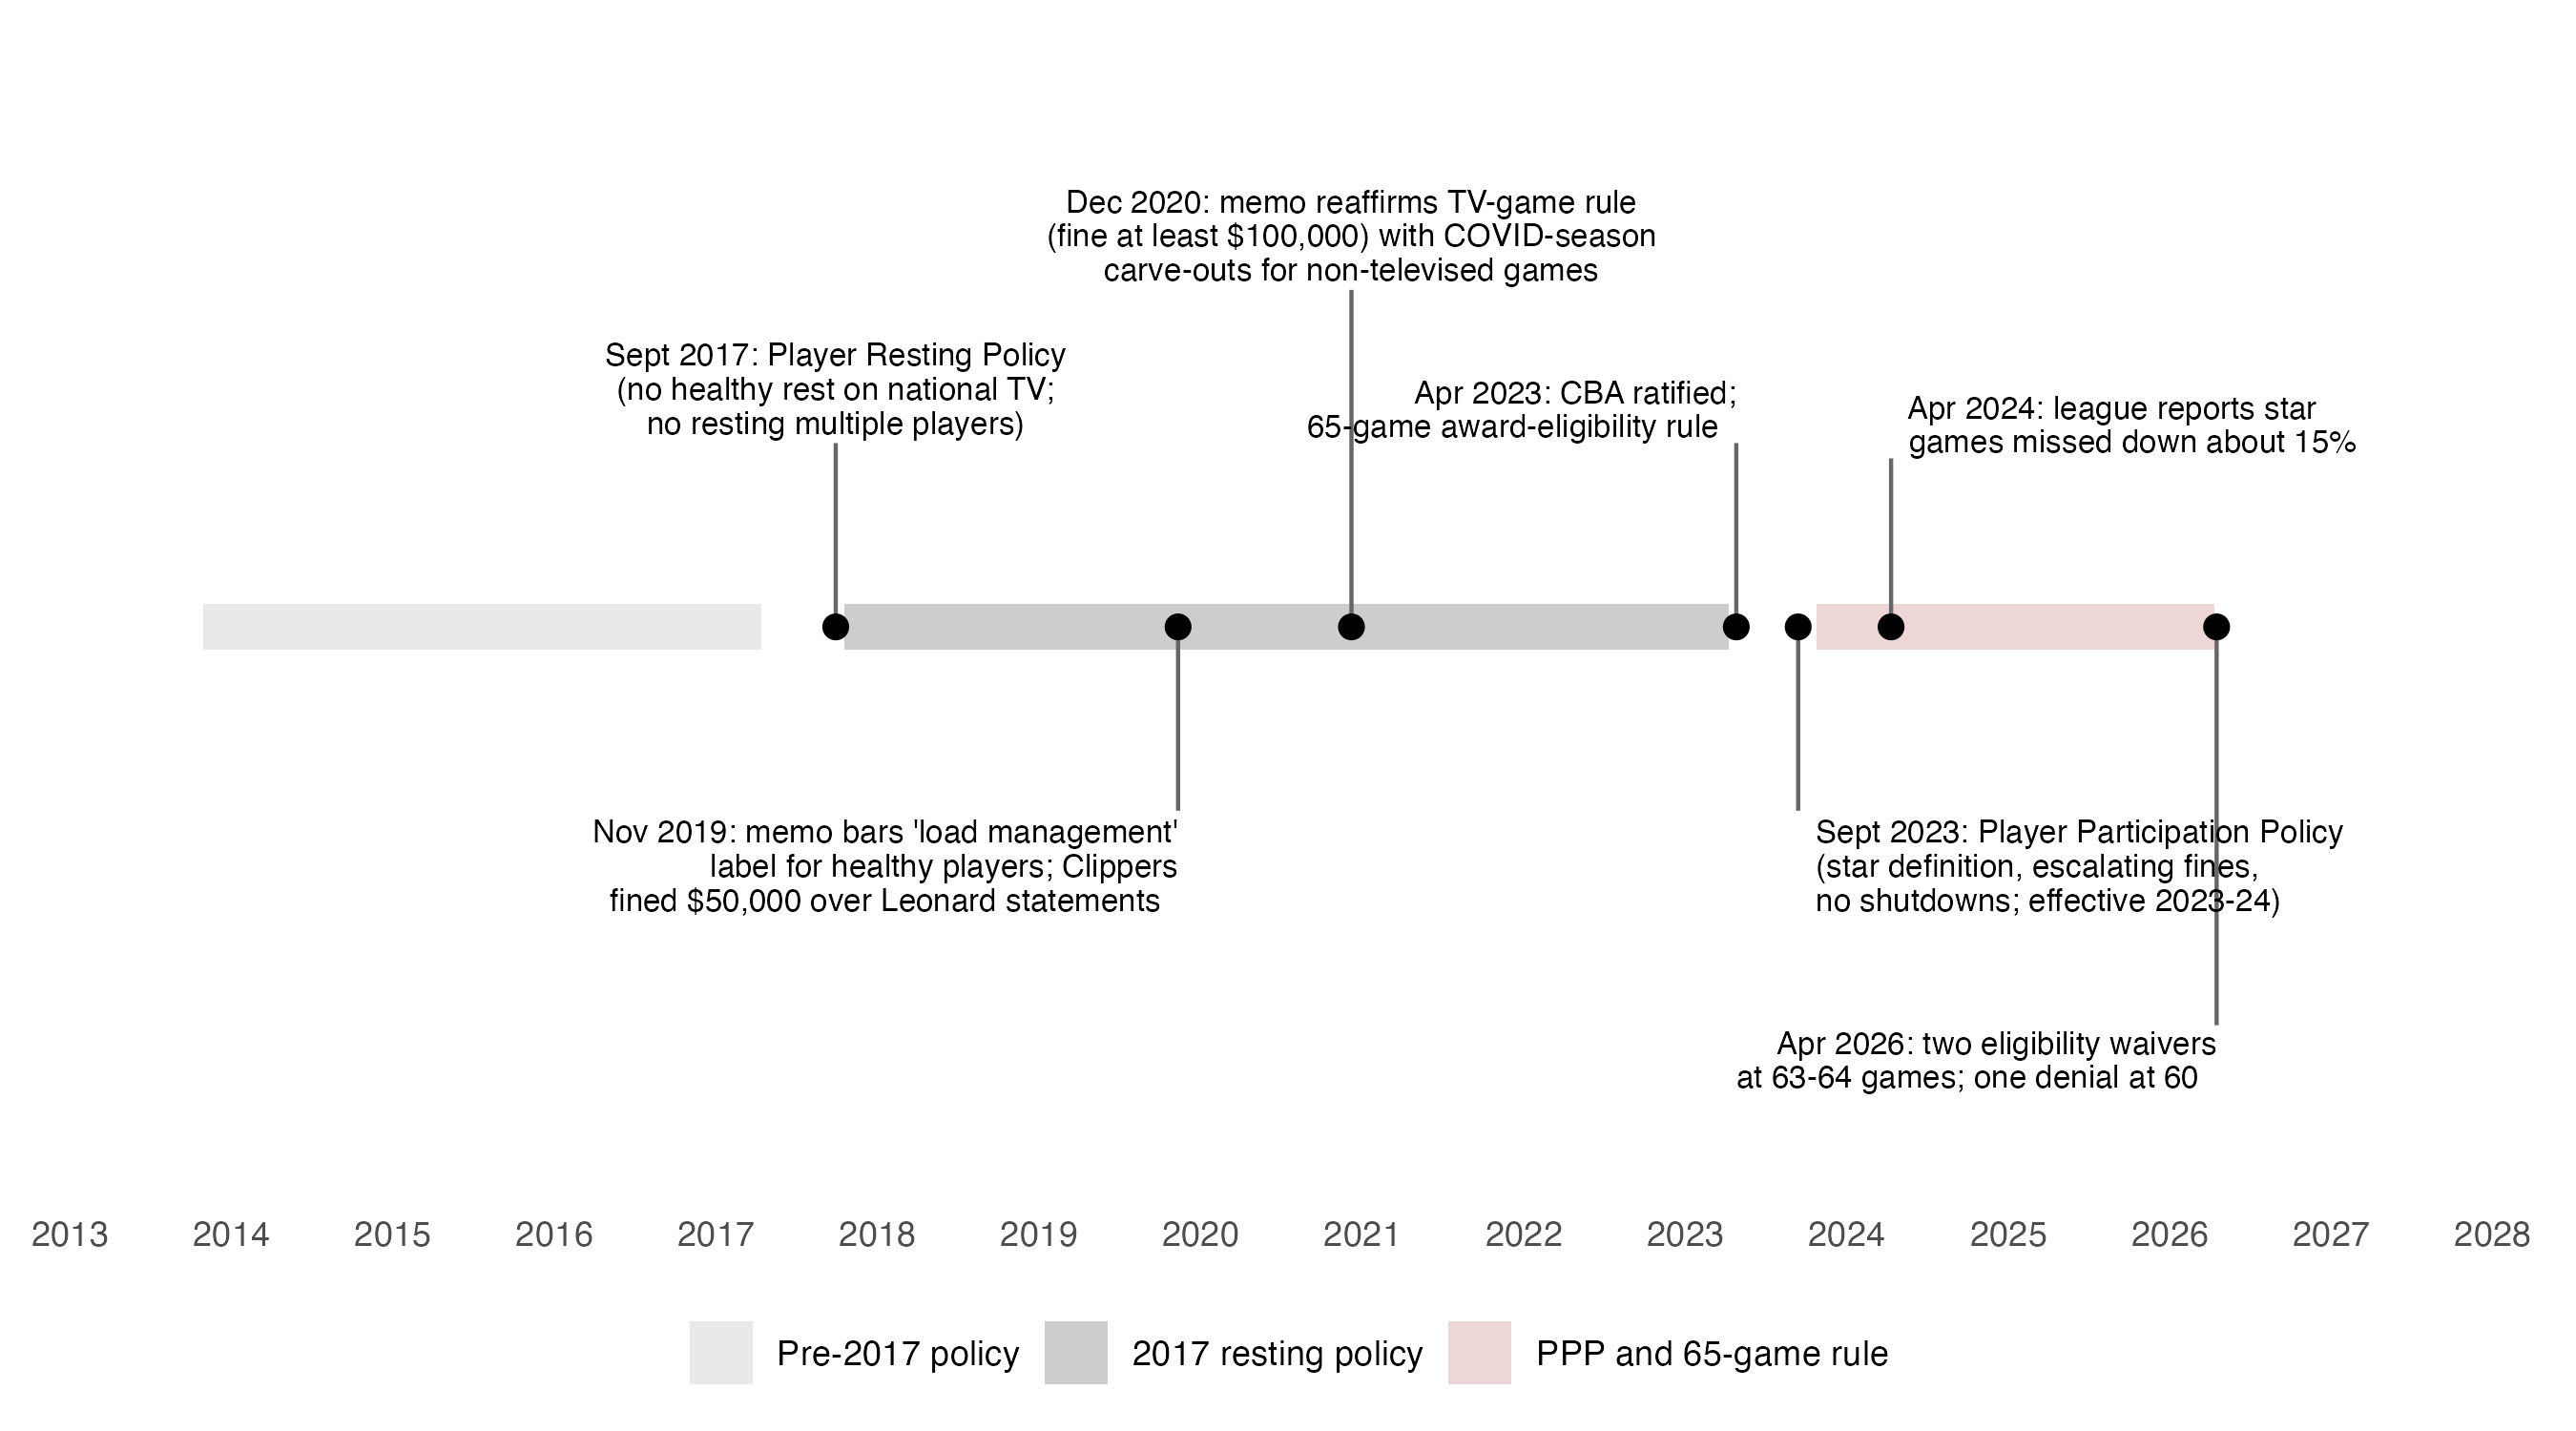
\includegraphics[width=\linewidth]{../../results/figures/paper/fig1_policy_timeline.png}
\caption{Policy timeline: the 2017 resting policy, the 2019 and 2020 memos, the 2023 CBA and Player Participation Policy, and the 2026 waivers. Shaded bars mark the regimes; 2019-20 and 2020-21 are excluded from estimation.}
\label{fig:fig1_policy_timeline}
\end{figure}

\begin{figure}[p]
\centering
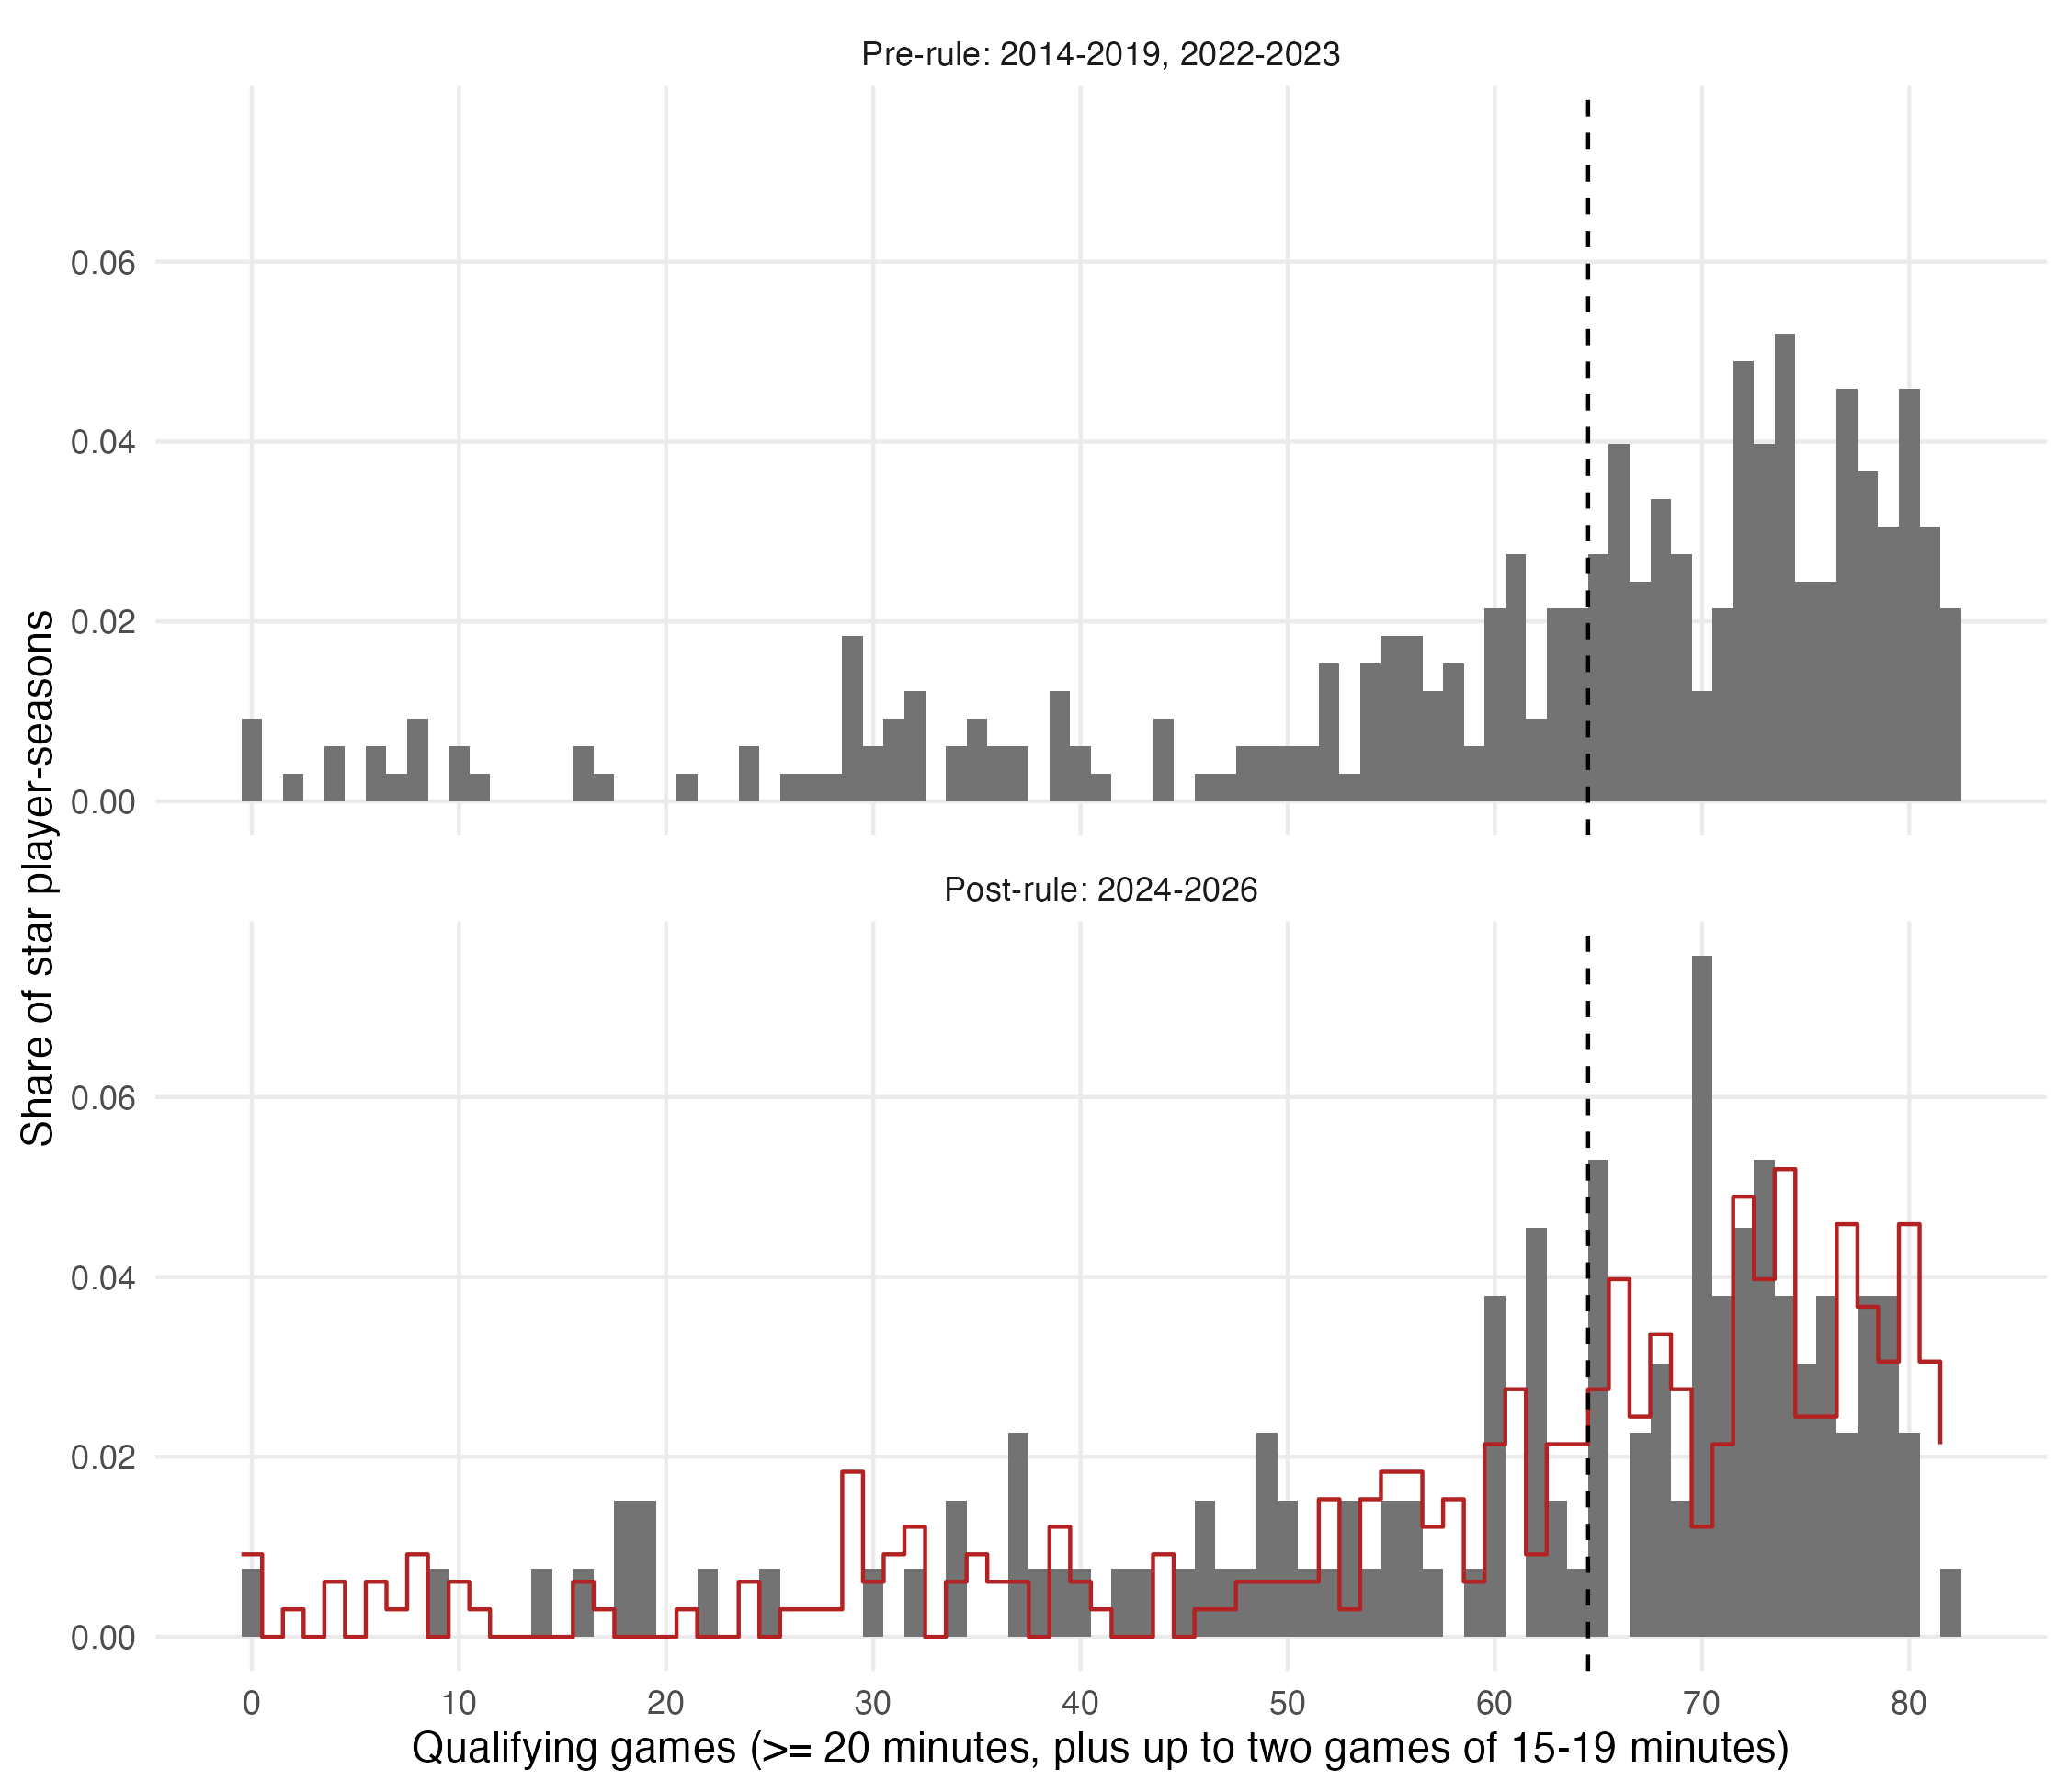
\includegraphics[width=\linewidth]{../../results/figures/paper/fig2_bunching_histogram.png}
\caption{Qualifying games of star player-seasons before and after the 65-game rule. Dashed line: 65-game threshold. Red step in the lower panel: pre-rule distribution scaled to the post-rule count (the counterfactual).}
\label{fig:fig2_bunching_histogram}
\end{figure}

\begin{figure}[p]
\centering
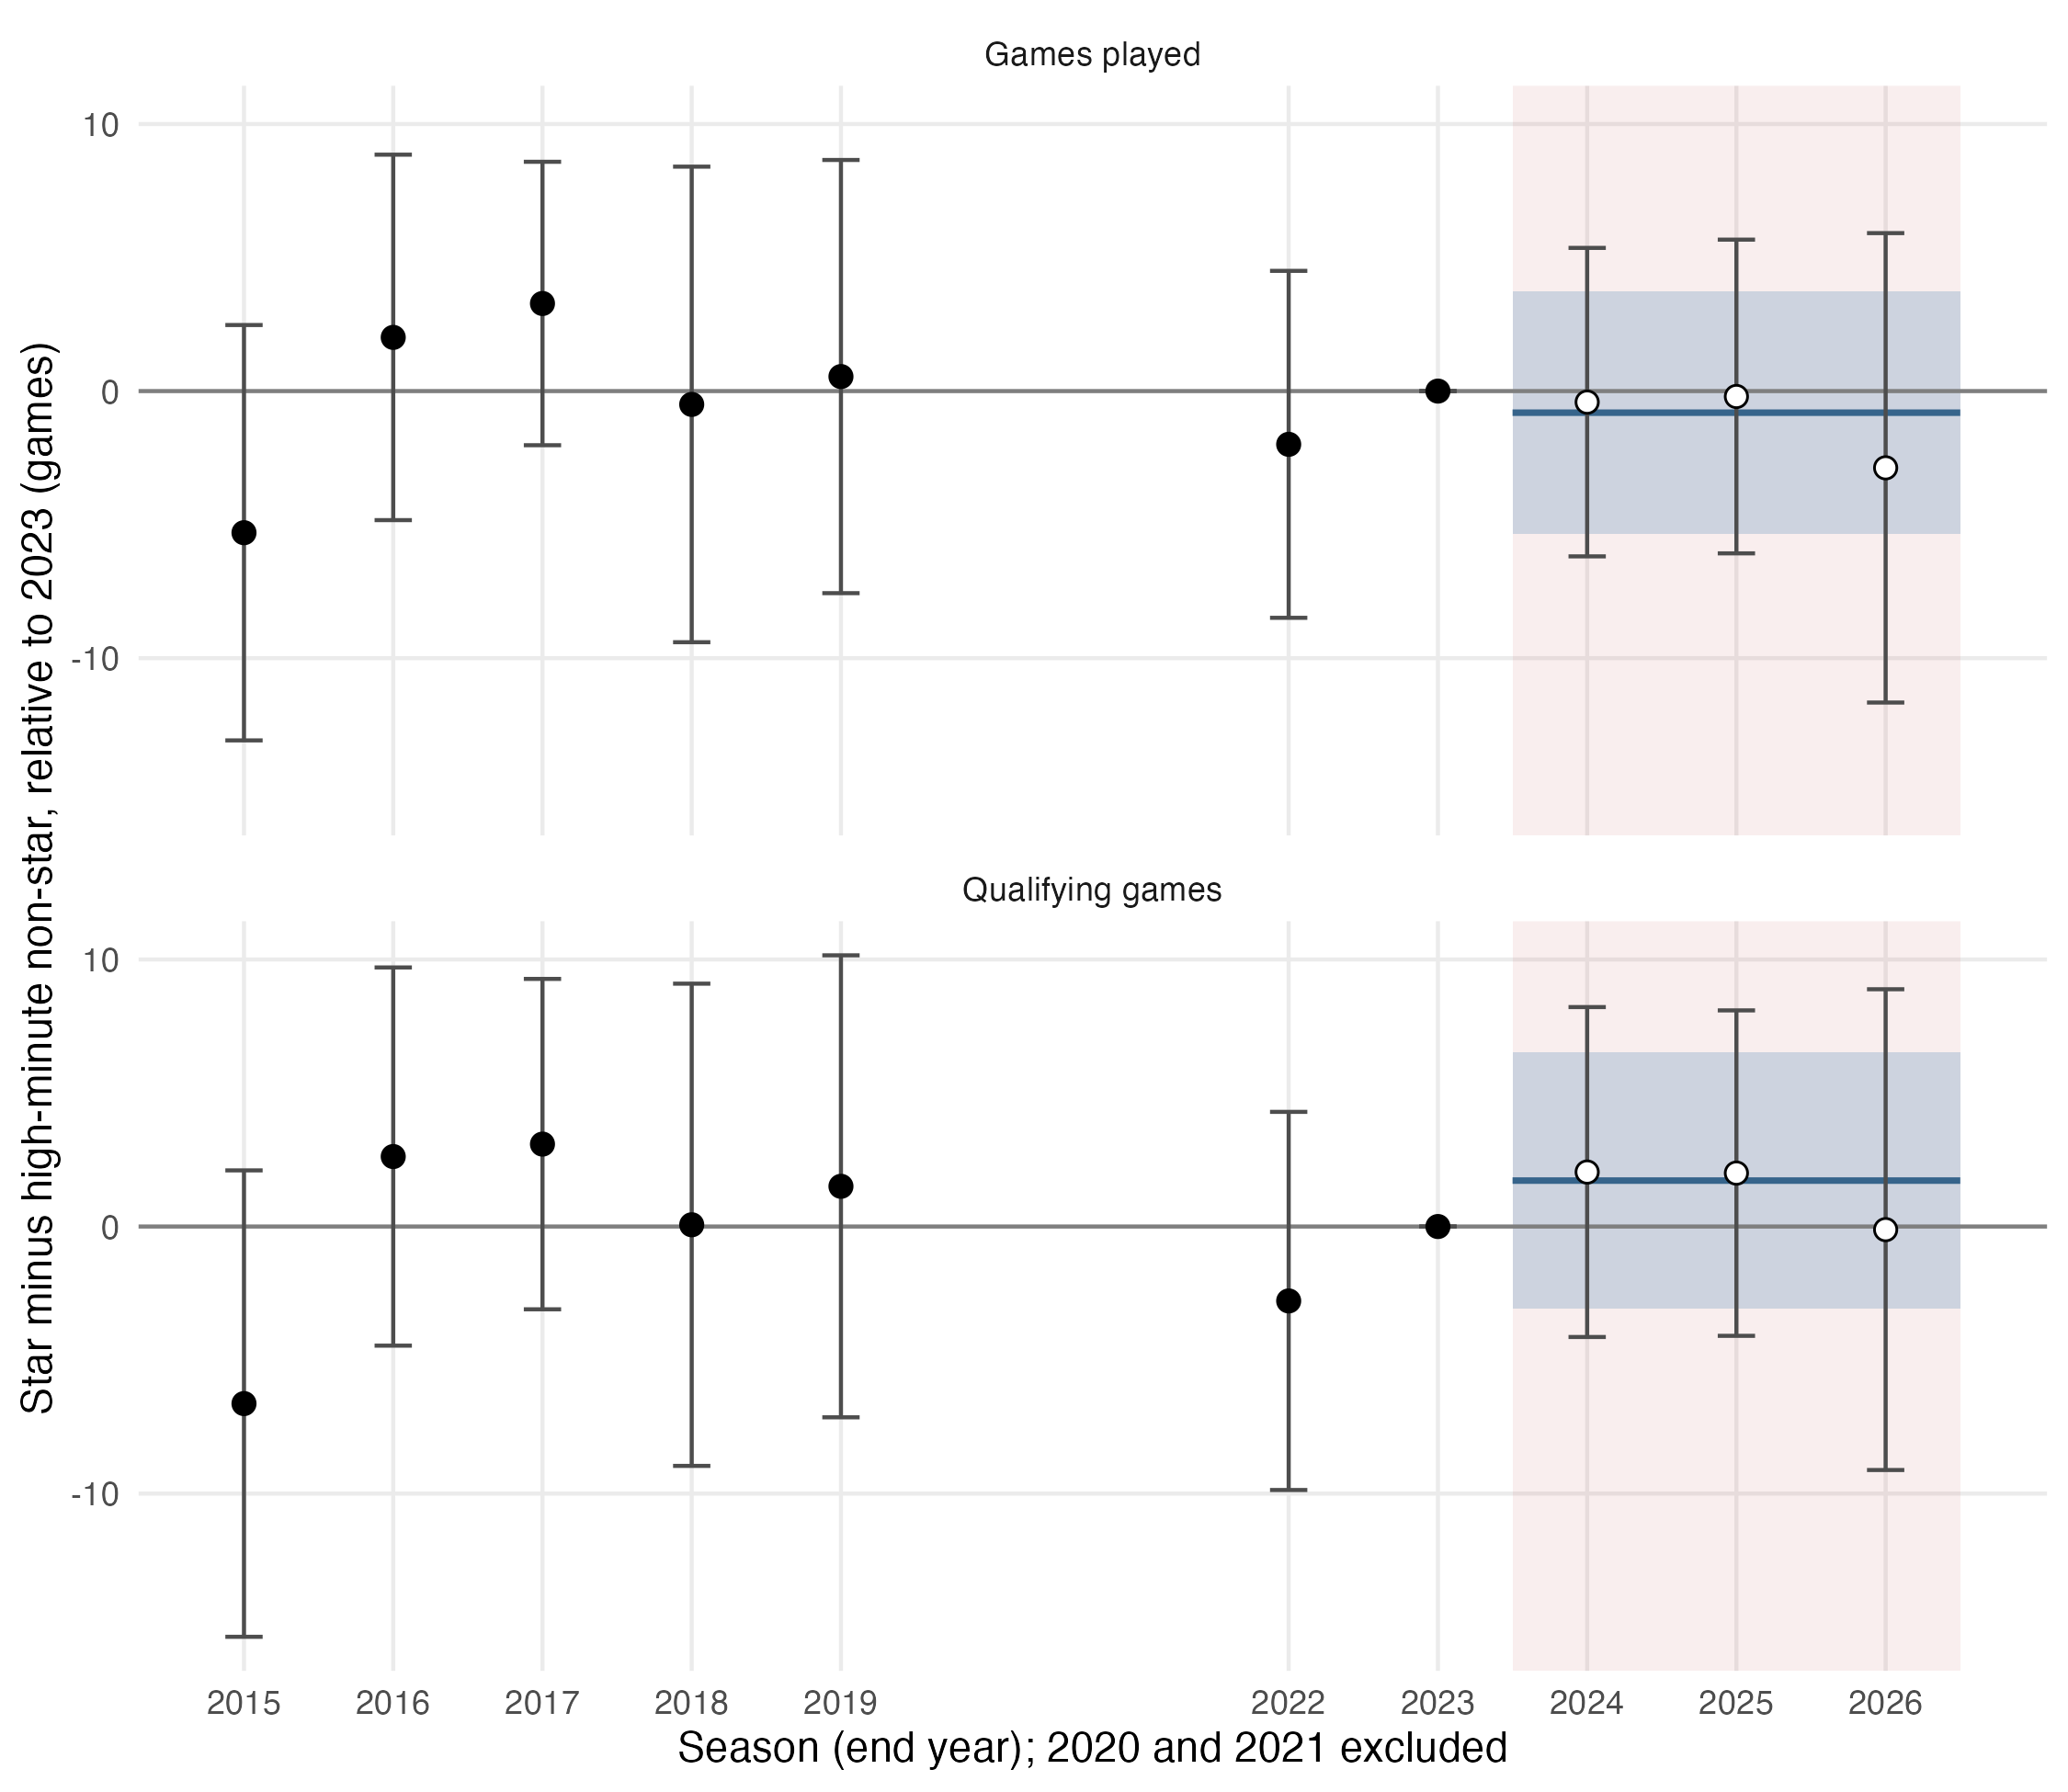
\includegraphics[width=\linewidth]{../../results/figures/paper/fig3_availability_event_study.png}
\caption{Star availability relative to high-minute non-stars defined on prior-season status, by season, reference 2023. Player and season fixed effects; 95 percent intervals clustered by player. Blue band: pooled post-rule estimate with its 95 percent interval.}
\label{fig:fig3_availability_event_study}
\end{figure}

\begin{figure}[p]
\centering
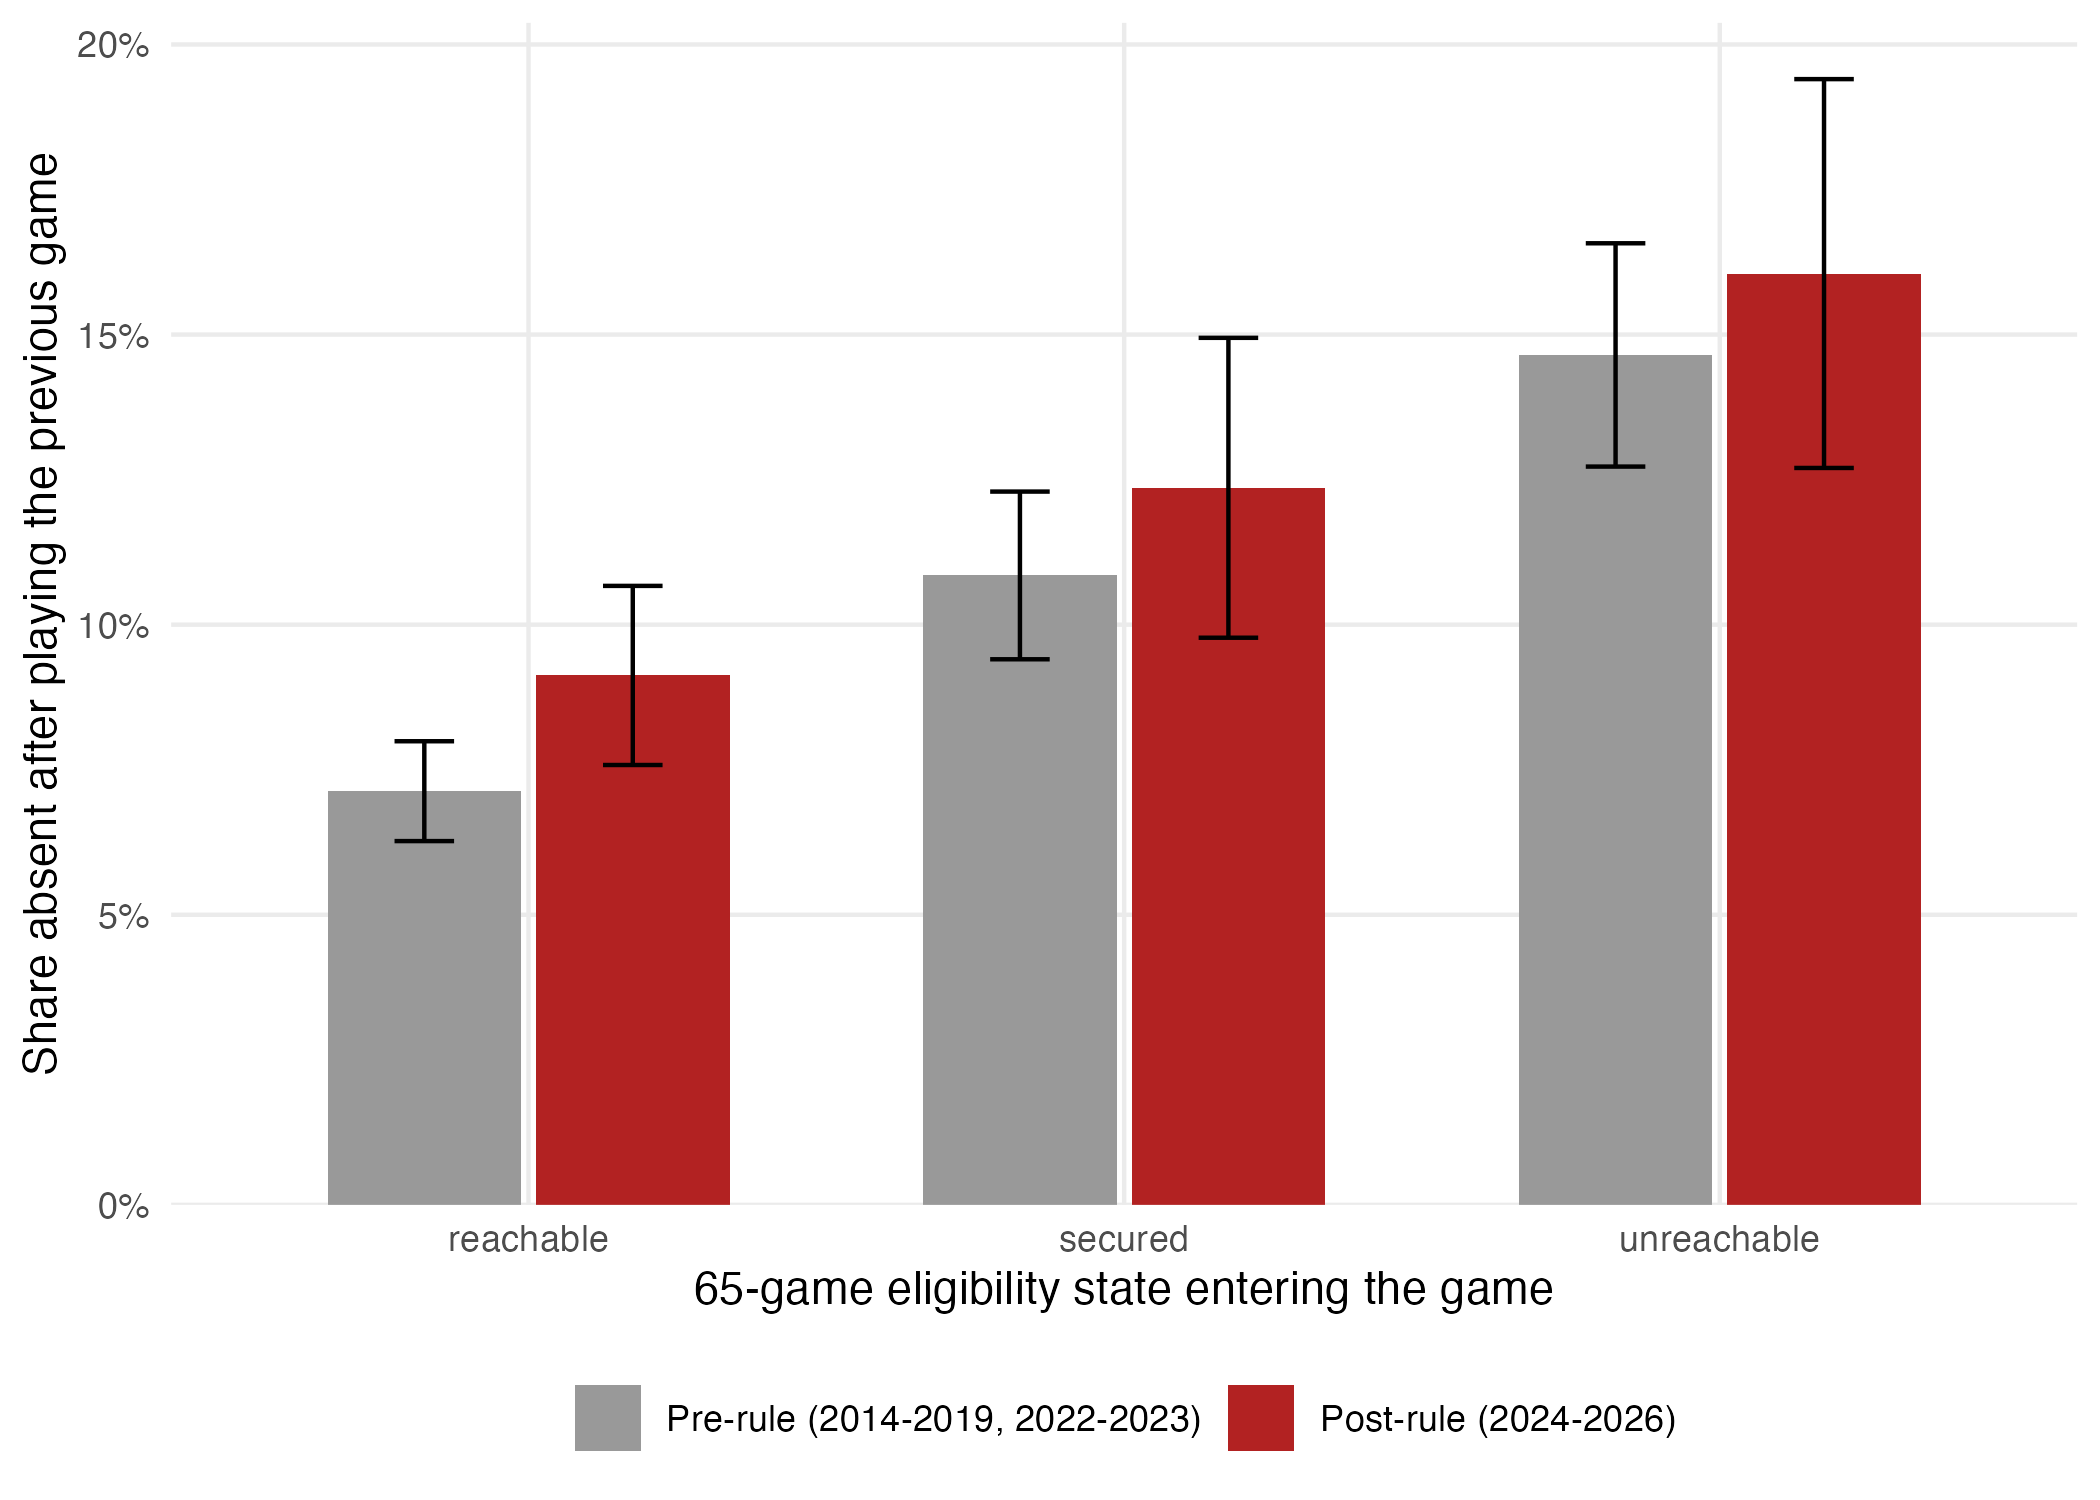
\includegraphics[width=\linewidth]{../../results/figures/paper/fig4_absence_by_state.png}
\caption{Late-season absence of stars who played the previous game, by eligibility state, before and after the rule, with 95 percent binomial intervals.}
\label{fig:fig4_absence_by_state}
\end{figure}

\begin{figure}[p]
\centering
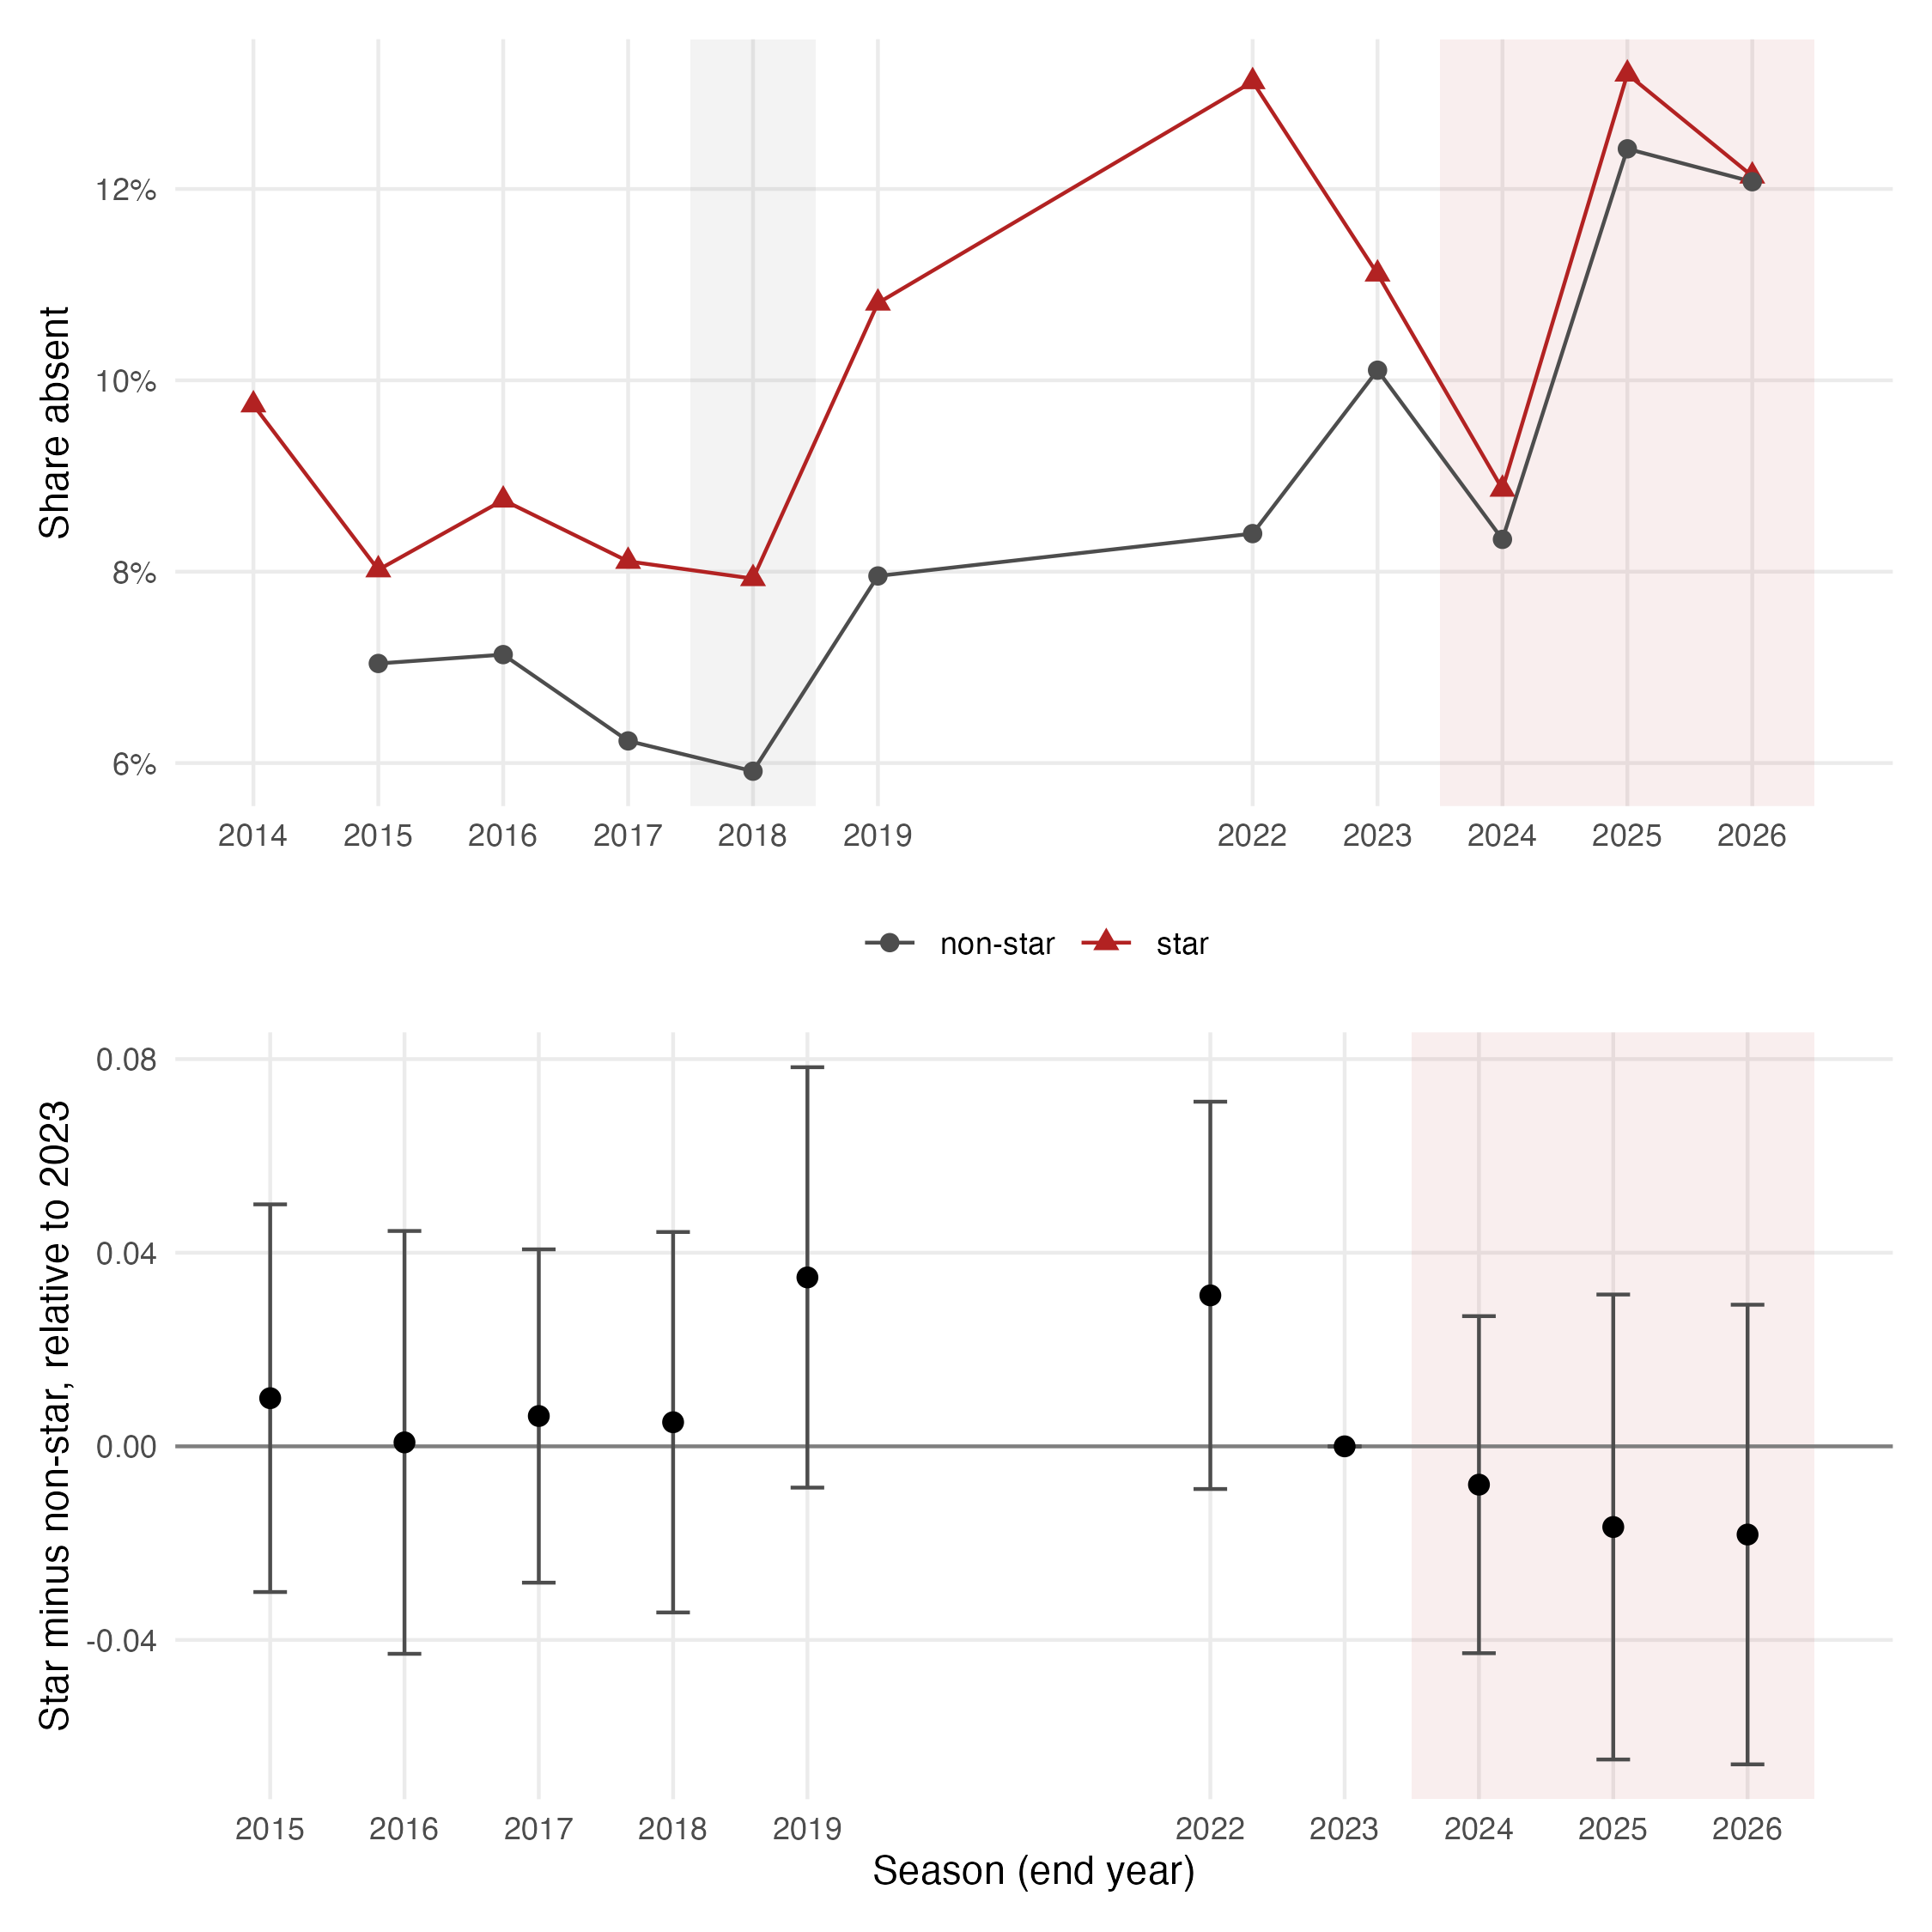
\includegraphics[width=\linewidth]{../../results/figures/paper/fig5_absence_stars_vs_nonstars.png}
\caption{Late-season absence after playing the previous game: stars and the control group. Upper panel: raw rates. Lower panel: star-by-season coefficients relative to 2023 with player, season and game-number fixed effects.}
\label{fig:fig5_absence_stars_vs_nonstars}
\end{figure}

\clearpage
\section*{Tables}
\begin{table}[!h]
\centering
\caption{\label{tab:tab1_sample}Sample by season: stars and the primary control group}
\centering
\resizebox{\ifdim\width>\linewidth\linewidth\else\width\fi}{!}{
\begin{threeparttable}
\begin{tabular}[t]{rlrrlllrrl}
\toprule
Season & Period & Stars & No appearance & Games played & Qualifying games & Share >= 65 & Contenders & High-minute non-stars (prior season) & Their games played\\
\midrule
2014 & Pre & 41 & 0 & 60.3 & 57.9 & 0.49 & 21 & 0 & \\
2015 & Pre & 43 & 1 & 63.2 & 60.9 & 0.65 & 22 & 88 & 66.4\\
2016 & Pre & 46 & 0 & 69.1 & 66.0 & 0.70 & 17 & 71 & 66.9\\
2017 & Pre & 40 & 3 & 70.2 & 66.3 & 0.65 & 20 & 79 & 65.9\\
2018 & Pre & 36 & 3 & 64.2 & 62.2 & 0.58 & 16 & 74 & 63.3\\
2019 & Pre & 37 & 1 & 63.1 & 61.6 & 0.65 & 20 & 72 & 64.2\\
2022 & Pre & 39 & 4 & 58.1 & 56.7 & 0.54 & 18 & 76 & 60.9\\
2023 & Pre & 45 & 0 & 59.4 & 58.4 & 0.44 & 17 & 82 & 65.6\\
2024 & Post & 46 & 0 & 65.0 & 64.5 & 0.67 & 19 & 90 & 66.1\\
2025 & Post & 46 & 0 & 62.4 & 62.0 & 0.54 & 19 & 81 & 62.0\\
2026 & Post & 40 & 2 & 54.8 & 54.4 & 0.47 & 16 & 68 & 58.8\\
\bottomrule
\end{tabular}
\begin{tablenotes}
\item \textit{Note: } 
\item Seasons indexed by end year; 2020 and 2021 excluded. Stars: All-Star or All-NBA in any of the prior three seasons (the PPP definition), with at least one ESPN box-score appearance. 'No appearance': flagged stars with no row in the season (retired or absent all season). All-Star and Rising Stars rows removed. Games played is the regular-season statistic and excludes the NBA Cup final; qualifying games follow the rule (>= 20 minutes plus up to two games of 15-19 minutes) and include the Cup final, so the two can differ by one for players on the finalist teams. Contenders: All-NBA or any MVP/DPOY vote in the prior season. High-minute non-stars: not a star in the season, and >= 28 minutes per game with >= 40 games played in the PRIOR season; none defined for 2014.
\end{tablenotes}
\end{threeparttable}}
\end{table}


\begin{table}[!h]
\centering
\caption{\label{tab:tab2_source_coverage}ESPN box-score coverage of absences, by season}
\centering
\resizebox{\ifdim\width>\linewidth\linewidth\else\width\fi}{!}{
\begin{threeparttable}
\begin{tabular}[t]{rrrllrrll}
\toprule
Season & Star team-games & Star absences & Star absence rate & Star absences with a DNP row & Non-star team-games & Non-star absences & Non-star absence rate & Non-star absences with a DNP row\\
\midrule
2014 & 3331 & 860 & 25.8\% & 29\% & NA & NA &  & \\
2015 & 3520 & 804 & 22.8\% & 28\% & 7211 & 1366 & 18.9\% & 30\%\\
2016 & 3769 & 590 & 15.7\% & 37\% & 5826 & 1074 & 18.4\% & 38\%\\
2017 & 3269 & 459 & 14.0\% & 40\% & 6444 & 1240 & 19.2\% & 35\%\\
2018 & 2945 & 634 & 21.5\% & 15\% & 6033 & 1348 & 22.3\% & 17\%\\
2019 & 3030 & 694 & 22.9\% & 15\% & 5860 & 1238 & 21.1\% & 16\%\\
2022 & 3193 & 927 & 29.0\% & 10\% & 6217 & 1588 & 25.5\% & 9\%\\
2023 & 3655 & 984 & 26.9\% & 7\% & 6710 & 1334 & 19.9\% & 17\%\\
2024 & 3773 & 781 & 20.7\% & 8\% & 7311 & 1351 & 18.5\% & 19\%\\
2025 & 3738 & 863 & 23.1\% & 16\% & 6603 & 1578 & 23.9\% & 23\%\\
2026 & 3250 & 1053 & 32.4\% & 10\% & 5524 & 1520 & 27.5\% & 22\%\\
\bottomrule
\end{tabular}
\begin{tablenotes}
\item \textit{Note: } 
\item Team-games: every regular-season game of the player's team stint(s). An absence is a team-game the player did not play. A DNP row is an ESPN box-score line for a player who did not play; it carries a reason string. Absences without a row carry no information beyond the fact of absence. Non-stars are high-minute non-stars by prior-season status.
\end{tablenotes}
\end{threeparttable}}
\end{table}


\begin{table}[!h]
\centering
\caption{\label{tab:tab3a_availability_event_study}Star availability relative to high-minute non-stars, by season (reference 2023)}
\centering
\resizebox{\ifdim\width>\linewidth\linewidth\else\width\fi}{!}{
\begin{threeparttable}
\begin{tabular}[t]{rllllll}
\toprule
Season & GP: est (SE) & GP: MDE & QG: est (SE) & QG: MDE & GP, rotation control: est (SE) & GP, rotation: MDE\\
\midrule
2015 & -5.30 (3.97) & 11.1 & -6.63 (4.46) & 12.5 & -5.18 (3.91) & 11.0\\
2016 & 2.01 (3.49) & 9.8 & 2.62 (3.61) & 10.1 & 2.20 (2.80) & 7.8\\
2017 & 3.28 (2.71) & 7.6 & 3.09 (3.16) & 8.8 & 5.10 (2.27) & 6.4\\
2018 & -0.50 (4.54) & 12.7 & 0.07 (4.61) & 12.9 & 0.22 (3.82) & 10.7\\
2019 & 0.54 (4.14) & 11.6 & 1.51 (4.41) & 12.4 & 0.76 (3.41) & 9.5\\
2022 & -1.99 (3.31) & 9.3 & -2.79 (3.61) & 10.1 & -0.31 (2.90) & 8.1\\
2023 & 0.00 (0.00) & 0.0 & 0.00 (0.00) & 0.0 & 0.00 (0.00) & 0.0\\
2024 & -0.41 (2.95) & 8.3 & 2.04 (3.15) & 8.8 & 3.49 (2.72) & 7.6\\
2025 & -0.20 (3.00) & 8.4 & 2.00 (3.11) & 8.7 & 4.25 (2.71) & 7.6\\
2026 & -2.87 (4.48) & 12.6 & -0.12 (4.59) & 12.9 & -0.68 (4.01) & 11.2\\
\bottomrule
\end{tabular}
\begin{tablenotes}
\item \textit{Note: } 
\item Outcomes: games played (GP) and qualifying games (QG) per player-season. Coefficients on star x season, player and season fixed effects, SEs clustered by player, 2020-2021 excluded, seasons 2015-2026, no filter on the outcome. Control groups are defined by prior-season status: high-minute (>= 28 minutes per game, >= 40 games) or rotation (>= 20 minutes, >= 40 games). MDE: minimum detectable effect at 80\% power and 5\% size (2.80 x SE), in games.
\end{tablenotes}
\end{threeparttable}}
\end{table}


\begin{table}[!h]
\centering
\caption{\label{tab:tab3b_availability_pooled}Pooled post-rule x star differences in availability}
\centering
\resizebox{\ifdim\width>\linewidth\linewidth\else\width\fi}{!}{
\begin{threeparttable}
\begin{tabular}[t]{lllllrr}
\toprule
Outcome & Control & Post x star: est (SE) & 95\% CI & MDE & Player-seasons & Players\\
\midrule
Games played & High-minute non-stars (prior season) & -0.809 (2.325) & {}[-5.37, 3.75] & 6.51 & 1093 & 255\\
Qualifying games & High-minute non-stars (prior season) & 1.720 (2.449) & {}[-3.08, 6.52] & 6.86 & 1093 & 255\\
Games played & Rotation non-stars (prior season) & 2.468 (2.142) & {}[-1.73, 6.67] & 6.00 & 2037 & 478\\
Qualifying games & Rotation non-stars (prior season) & 6.814 (2.302) & {}[2.30, 11.33] & 6.45 & 2037 & 478\\
Games played & Exploratory: contemporaneous control, >= 40 rostered games & 1.048 (1.412) & {}[-1.72, 3.82] & 3.96 & 1194 & 274\\
Qualifying games & Exploratory: contemporaneous control, >= 40 rostered games & 0.942 (1.428) & {}[-1.86, 3.74] & 4.00 & 1194 & 274\\
Share >= 65 & High-minute non-stars (prior season) & 0.067 (0.070) & {}[-0.07, 0.20] & 0.20 & 1093 & 255\\
\bottomrule
\end{tabular}
\begin{tablenotes}
\item \textit{Note: } 
\item Post-rule = 2024-2026. Player and season fixed effects; SEs clustered by player. MDE at 80\% power. The exploratory row conditions the control on games played >= 40 in the same season and drops player-seasons with fewer than 40 ESPN rows, which removes stars' long-injury seasons; it is shown for comparison only.
\end{tablenotes}
\end{threeparttable}}
\end{table}


\begin{table}[!h]
\centering
\caption{\label{tab:tab4a_bunching_bins}Star player-seasons around the 65-game threshold, pre- vs post-rule}
\centering
\resizebox{\ifdim\width>\linewidth\linewidth\else\width\fi}{!}{
\begin{threeparttable}
\begin{tabular}[t]{lrlrl}
\toprule
Qualifying games & Pre: n & Pre: share & Post: n & Post: share\\
\midrule
<58 & 95 & 0.291 & 42 & 0.318\\
58-64 (below) & 40 & 0.122 & 15 & 0.114\\
65-68 (just above) & 41 & 0.125 & 14 & 0.106\\
69+ & 151 & 0.462 & 61 & 0.462\\
\bottomrule
\end{tabular}
\begin{tablenotes}
\item \textit{Note: } 
\item Stars, 2020-2021 excluded. Pre-rule 2014-2019 and 2022-2023; post-rule 2024-2026.
\end{tablenotes}
\end{threeparttable}}
\end{table}


\begin{table}[!h]
\centering
\caption{\label{tab:tab4b_bunching_excess_mass}Excess mass at and above 65 qualifying games, post-rule stars}
\centering
\resizebox{\ifdim\width>\linewidth\linewidth\else\width\fi}{!}{
\begin{threeparttable}
\begin{tabular}[t]{llllllll}
\toprule
Counterfactual & Window & Above: observed & Above: counterfactual & b (95\% CI) & Below: observed & Below: counterfactual & m (95\% CI)\\
\midrule
All pre-rule seasons & 65 vs 64 & 7 & 3.6 & 0.93 [-0.38, 4.57] & 1 & 2.8 & -0.65 [-1.00, 0.86]\\
All pre-rule seasons & 65-66 vs 63-64 & 7 & 8.9 & -0.42 [-1.45, 1.30] & 3 & 5.7 & -0.94 [-2.00, 1.05]\\
All pre-rule seasons & 65-68 vs 58-64 & 14 & 16.6 & -0.62 [-2.24, 1.81] & 15 & 16.1 & -0.50 [-3.53, 3.90]\\
2022-2023 only & 65 vs 64 & 7 & 9.4 & -0.26 [-0.76, 1.55] & 1 & 3.1 & -0.68 [-1.00, 0.91]\\
2022-2023 only & 65-66 vs 63-64 & 7 & 18.9 & -1.26 [-1.77, -0.18] & 3 & 6.3 & -1.05 [-2.00, 3.09]\\
2022-2023 only & 65-68 vs 58-64 & 14 & 31.4 & -2.22 [-3.11, -0.76] & 15 & 15.7 & -0.32 [-3.86, 9.04]\\
\bottomrule
\end{tabular}
\begin{tablenotes}
\item \textit{Note: } 
\item Counterfactual: the pre-rule distribution of stars' qualifying games scaled to the post-rule count. b = excess player-seasons in the window above 65 divided by the mean counterfactual mass per one-game bin in that window; m likewise for the window below. 95\% CIs from 2,000 bootstrap resamples of both distributions.
\end{tablenotes}
\end{threeparttable}}
\end{table}


\begin{table}[!h]
\centering
\caption{\label{tab:tab5a_at_risk_reach}Healthy at-risk stars at team game 62: did they reach 65?}
\centering
\resizebox{\ifdim\width>\linewidth\linewidth\else\width\fi}{!}{
\begin{threeparttable}
\begin{tabular}[t]{lrlrll}
\toprule
Slack at game 62 & Pre: n & Pre: reached 65 & Post: n & Post: reached 65 & Fisher p\\
\midrule
0-2 & 20 & 0.40 & 2 & 1.00 & 0.19\\
3-5 & 27 & 0.70 & 8 & 0.62 & 0.69\\
6-8 & 25 & 0.60 & 11 & 0.64 & 1.00\\
\bottomrule
\end{tabular}
\begin{tablenotes}
\item \textit{Note: } 
\item At risk: 0-8 games of slack at team game 62 (qualifying games so far plus games left minus 65). Healthy: played at least two of games 60-62. Reached: >= 65 qualifying games at season end. Fisher exact test of pre vs post.
\end{tablenotes}
\end{threeparttable}}
\end{table}


\begin{table}[!h]
\centering
\caption{\label{tab:tab5b_at_risk_regressions}Post-rule change in the probability that an at-risk star reaches 65}
\centering
\resizebox{\ifdim\width>\linewidth\linewidth\else\width\fi}{!}{
\begin{threeparttable}
\begin{tabular}[t]{lrrllll}
\toprule
Sample & n & Post n & Pre reach & Post reach & Post: est (SE) & MDE\\
\midrule
All at-risk stars & 116 & 34 & 0.56 & 0.53 & -0.05 (0.10) & 0.28\\
Healthy at game 62 & 93 & 21 & 0.58 & 0.67 & 0.06 (0.13) & 0.35\\
Healthy, with current-season contention control & 93 & 21 & 0.58 & 0.67 & 0.14 (0.13) & 0.36\\
Healthy, slack 0-5 & 57 & 10 & 0.57 & 0.70 & 0.13 (0.17) & 0.48\\
\bottomrule
\end{tabular}
\begin{tablenotes}
\item \textit{Note: } 
\item Linear probability models with slack-bin controls; SEs clustered by player. MDE at 80\% power, in probability points.
\end{tablenotes}
\end{threeparttable}}
\end{table}


\begin{table}[!h]
\centering
\caption{\label{tab:tab5c_bound}The maximal-effect bound on star mean qualifying games}
\centering
\resizebox{\ifdim\width>\linewidth\linewidth\else\width\fi}{!}{
\begin{threeparttable}
\begin{tabular}[t]{lllllll}
\toprule
Period & Stars per season & At risk per season & Share at risk & Did not reach & Bound, minimal crossing & Bound, play every game\\
\midrule
Post-rule (3 seasons) & 44.0 & 11.3 & 0.26 & 5.3 & 0.96 & 1.85\\
Pre-rule (8 seasons) & 40.9 & 10.2 & 0.25 & 4.5 & 0.67 & 1.27\\
\bottomrule
\end{tabular}
\begin{tablenotes}
\item \textit{Note: } 
\item Minimal crossing: every at-risk star who fell short instead reaches exactly 65. Play every game: every at-risk star plays every remaining game. Both divided by the number of stars that season and averaged over seasons; units are games per star player-season.
\end{tablenotes}
\end{threeparttable}}
\end{table}


\begin{table}[!h]
\centering
\caption{\label{tab:tab5d_case_table}Healthy at-risk stars in the post-rule seasons: slack at game 62, outcome, return minutes, and stakes}
\centering
\resizebox{\ifdim\width>\linewidth\linewidth\else\width\fi}{!}{
\begin{threeparttable}
\begin{tabular}[t]{rlrrllrrrlll}
\toprule
season & player & slack\_at\_62 & qualifying\_thru\_62 & contender\_prior\_season & reached\_65 & final\_qualifying\_games & last\_absence\_before\_62 & absences\_before\_62 & minutes\_first\_4\_after\_return & received\_award\_votes & stakes\\
\midrule
2024 & Andrew Wiggins & 4 & 49 & FALSE & TRUE & 67 & 60 & 9 & 14, 15, 26, 30 & FALSE & none identified\\
2024 & Tyrese Haliburton & 4 & 48 & FALSE & TRUE & 69 & 48 & 13 & 22, 22, 22, 20 & TRUE & Rose Rule: 2023 rookie extension worth 30\% of cap instead of 25\% with All-NBA in 2024 (about \$40M); made All-NBA Third Team\\
2024 & Bam Adebayo & 6 & 51 & TRUE & TRUE & 70 & 26 & 10 & 36, 30, 38, 36 & TRUE & All-NBA in 2024 would have made him eligible for a Designated Veteran (35\%) extension, four years and about \$245M versus the three-year \$165M deal otherwise available; not selected\\
2024 & Lauri Markkanen & 6 & 51 & FALSE & FALSE & 55 & 29 & 10 & 39, 31, 35, 26 & FALSE & none identified\\
2024 & Zion Williamson & 6 & 51 & FALSE & TRUE & 70 & 53 & 11 & 35, 34, 35, 36 & TRUE & Guarantees for 2025-26 onward keyed to games played: 40\% at 41 games, a further 20\% at 51, full at 61, plus weigh-in criteria; later years had become non-guaranteed after 53 missed games in 2022-23\\
2025 & Scottie Barnes & 3 & 48 & FALSE & TRUE & 65 & 59 & 14 & 36, 29, 30, 32 & FALSE & 2024 rookie extension projected at \$224.2M, rising to \$269.1M if Rose Rule criteria are met; not selected\\
2025 & Kevin Durant & 4 & 49 & TRUE & FALSE & 62 & 52 & 13 & 43, 42, 39, 38 & FALSE & none identified\\
2025 & Kyrie Irving & 4 & 49 & FALSE & FALSE & 49 & 56 & 12 & 37, 32, 40, 38 & FALSE & none identified\\
2025 & Giannis Antetokounmpo & 6 & 50 & TRUE & TRUE & 68 & 54 & 12 & 24, 19, 32, 32 & TRUE & none identified\\
2025 & Jaylen Brown & 7 & 52 & FALSE & FALSE & 63 & 59 & 10 & 34, 37, 40, 42 & FALSE & none identified; super-max signed July 2023, so no escalator\\
2025 & Damian Lillard & 8 & 52 & FALSE & FALSE & 59 & 56 & 10 & 38, 37, 35, 36 & FALSE & none identified\\
2025 & Stephen Curry & 8 & 53 & TRUE & TRUE & 70 & 46 & 9 & 33, 31, 34, 35 & TRUE & none identified\\
2026 & Nikola Jokic & 1 & 46 & TRUE & TRUE & 65 & 48 & 16 & 25, 29, 33, 45 & TRUE & none identified\\
2026 & Evan Mobley & 2 & 47 & TRUE & TRUE & 65 & 60 & 15 & 37, 27, 32, 31 & TRUE & Rose Rule already triggered by 2025 Defensive Player of the Year; no further stake in 2026\\
2026 & Kawhi Leonard & 3 & 48 & FALSE & TRUE & 65 & 58 & 14 & 29, 29, 23, 37 & TRUE & none identified\\
2026 & Victor Wembanyama & 4 & 48 & FALSE & TRUE & 65 & 36 & 14 & 21, 26, 26, 27 & TRUE & Rookie scale; All-NBA in 2026 counts toward Rose Rule criteria (preceding season, or two of the prior three) for his 2027 extension\\
2026 & Luka Doncic & 5 & 50 & FALSE & FALSE & 64 & 54 & 12 & 38, 33, 38, 39 & TRUE & Three-year max extension signed Aug 2025, projected \$160.4M; no escalator (eligibility by waiver)\\
2026 & Anthony Edwards & 6 & 51 & TRUE & FALSE & 60 & 47 & 10 & 38, 35, 39, 40 & FALSE & Rose Rule triggered by 2024 All-NBA; a 2026 All-NBA counts toward Designated Veteran criteria, but he lacks the years of service for a super-max extension until 2027; eligibility denied by arbitrator at 60\\
2026 & Paolo Banchero & 6 & 51 & FALSE & TRUE & 71 & 22 & 10 & 20, 24, 32, 35 & FALSE & 2025 rookie extension projected at \$239.25M, rising to \$287.1M with All-NBA, MVP or DPOY in 2025-26\\
2026 & Shai Gilgeous-Alexander & 6 & 51 & TRUE & TRUE & 68 & 60 & 11 & 34, 33, 35, 35 & TRUE & Super-max signed July 2025, projected \$284.6M; no escalator at stake\\
2026 & Bam Adebayo & 8 & 53 & TRUE & TRUE & 72 & 32 & 8 & 21, 33, 34, 29 & TRUE & Three-year max extension signed 2024, projected \$165.3M; no award terms\\
\bottomrule
\end{tabular}
\begin{tablenotes}
\item \textit{Note: } 
\item At risk: 0-8 games of slack at team game 62; healthy: played at least two of games 60-62. Return minutes: minutes in the first four appearances after the player's last absence before team game 62. Stakes are hand-coded from press coverage and the CBA; entries marked for verification in the csv should be checked against Spotrac before use.
\end{tablenotes}
\end{threeparttable}}
\end{table}


\begin{table}[!h]
\centering
\caption{\label{tab:tab6a_absence_by_state}Absence of stars who played the previous game, late season, by eligibility state}
\centering
\resizebox{\ifdim\width>\linewidth\linewidth\else\width\fi}{!}{
\begin{threeparttable}
\begin{tabular}[t]{lrlrllll}
\toprule
State & Pre: n & Pre: absent & Post: n & Post: absent & Change (SE) & Pre: with DNP row & Post: with DNP row\\
\midrule
reachable & 3436 & 7.1\% & 1337 & 9.1\% & 2.0 (0.9) & 2.7\% & 2.1\%\\
secured & 1779 & 10.8\% & 623 & 12.4\% & 1.5 (1.5) & 5.7\% & 2.1\%\\
unreachable & 1297 & 14.6\% & 461 & 16.1\% & 1.4 (2.0) & 6.7\% & 2.4\%\\
\bottomrule
\end{tabular}
\begin{tablenotes}
\item \textit{Note: } 
\item Games 56 onward, full team schedule, 2020-2021 excluded. Absent: did not play, whether or not ESPN printed a row. 'With DNP row': the part of the absence rate for which ESPN printed a row with a reason. Change in percentage points with a binomial SE.
\end{tablenotes}
\end{threeparttable}}
\end{table}


\begin{table}[!h]
\centering
\caption{\label{tab:tab6b_absence_state_regressions}State x post-rule regressions of late-season absence, stars}
\centering
\resizebox{\ifdim\width>\linewidth\linewidth\else\width\fi}{!}{
\begin{threeparttable}
\begin{tabular}[t]{lllll}
\toprule
Specification & Term & Est (SE) & p & MDE\\
\midrule
state main effects + state x post & secured & 0.006 (0.013) & 0.61 & 0.036\\
state main effects + state x post & secured x post & -0.011 (0.019) & 0.56 & 0.053\\
no-incentive + no-incentive x post & no incentive & -0.004 (0.012) & 0.73 & 0.034\\
no-incentive + no-incentive x post & no incentive x post & -0.005 (0.019) & 0.78 & 0.053\\
\bottomrule
\end{tabular}
\begin{tablenotes}
\item \textit{Note: } 
\item Player-season and team-game-number fixed effects; SEs clustered by player. Reference state: reachable. MDE at 80\% power. The unreachable state is omitted: within a player-season its games follow a long absence, so the within-player contrast is mechanically negative and the post interaction is identified from few transitions; Table 6a carries that state.
\end{tablenotes}
\end{threeparttable}}
\end{table}


\begin{table}[!h]
\centering
\caption{\label{tab:tab6c_absence_star_vs_nonstar}Star-specific change in late-season absence at the 2017 policy and the 2023 rule}
\centering
\resizebox{\ifdim\width>\linewidth\linewidth\else\width\fi}{!}{
\begin{threeparttable}
\begin{tabular}[t]{lrlll}
\toprule
Window & Player-games & Est (SE) & 95\% CI & MDE\\
\midrule
2014-2026: post-rule (2024-26) x star & 24606 & -0.019 (0.016) & {}[-0.050, 0.012] & 0.044\\
2022-2026: post-rule (2024-26) x star & 11807 & -0.023 (0.015) & {}[-0.053, 0.008] & 0.043\\
2014-2019: post-2017-policy (2018-19) x star & 12799 & 0.010 (0.016) & {}[-0.022, 0.041] & 0.045\\
\bottomrule
\end{tabular}
\begin{tablenotes}
\item \textit{Note: } 
\item Stars vs high-minute non-stars who played the previous game, games 56 onward, full schedule. Player, season and team-game-number fixed effects; SEs clustered by player. MDE at 80\% power.
\end{tablenotes}
\end{threeparttable}}
\end{table}


\clearpage
\appendix
\section*{Appendix figures}
\begin{figure}[p]
\centering
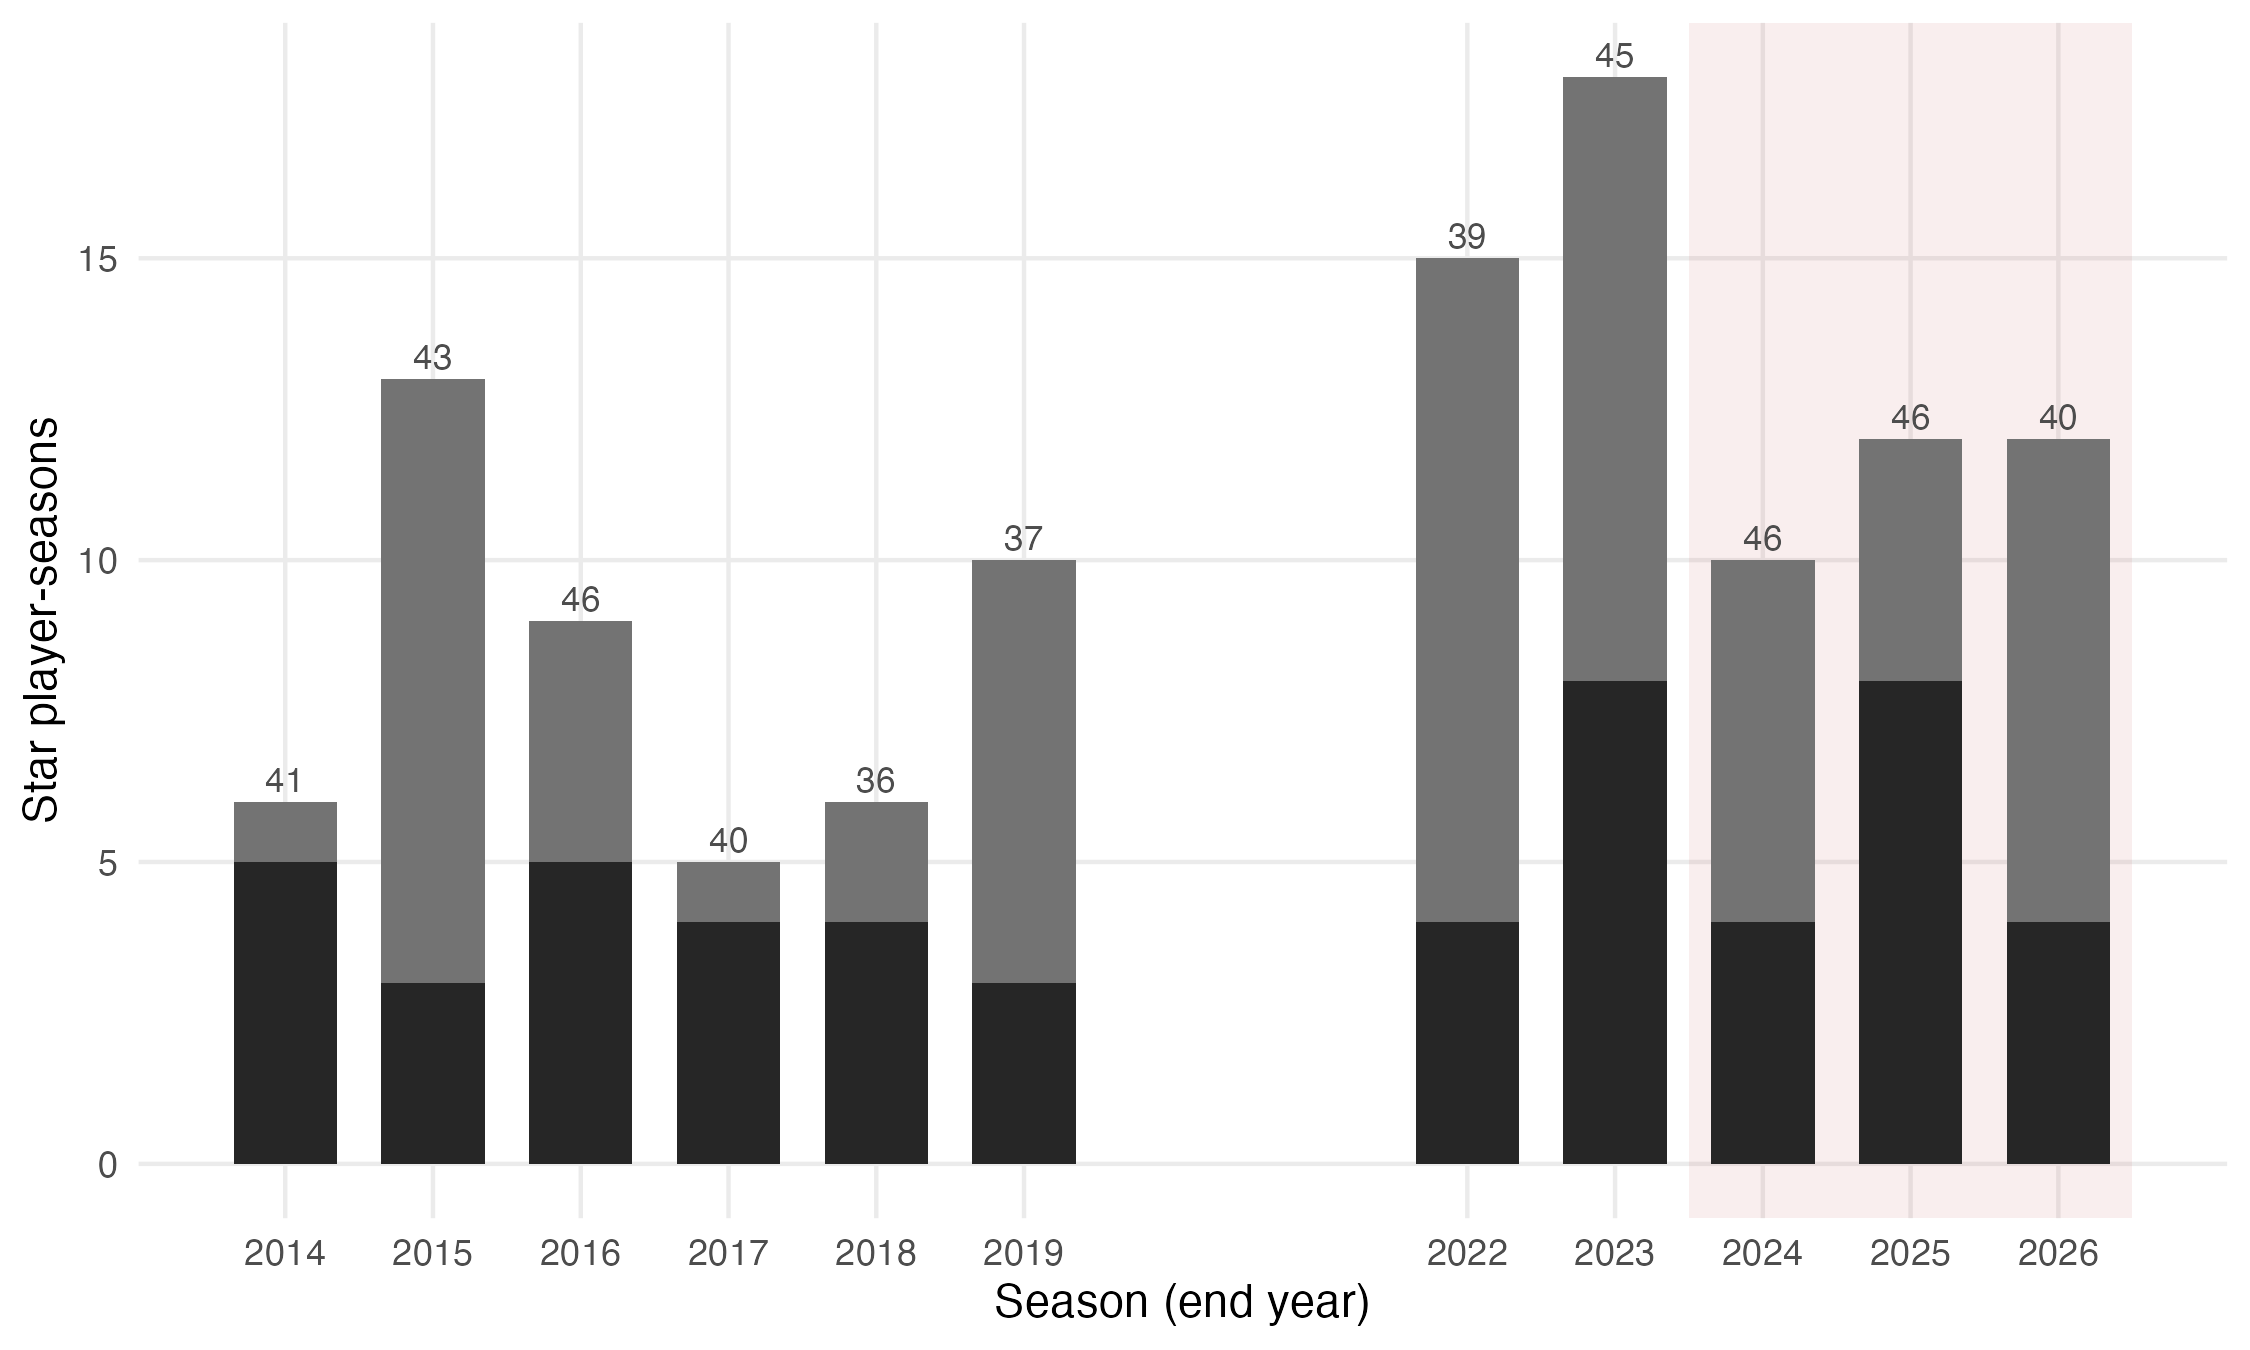
\includegraphics[width=\linewidth]{../../results/figures/paper/figA1_at_risk_by_season.png}
\caption{Stars at risk at team game 62 (slack 0-8), by season; black: at risk and did not reach 65; number above bar: stars that season.}
\label{fig:figA1_at_risk_by_season}
\end{figure}

\begin{figure}[p]
\centering
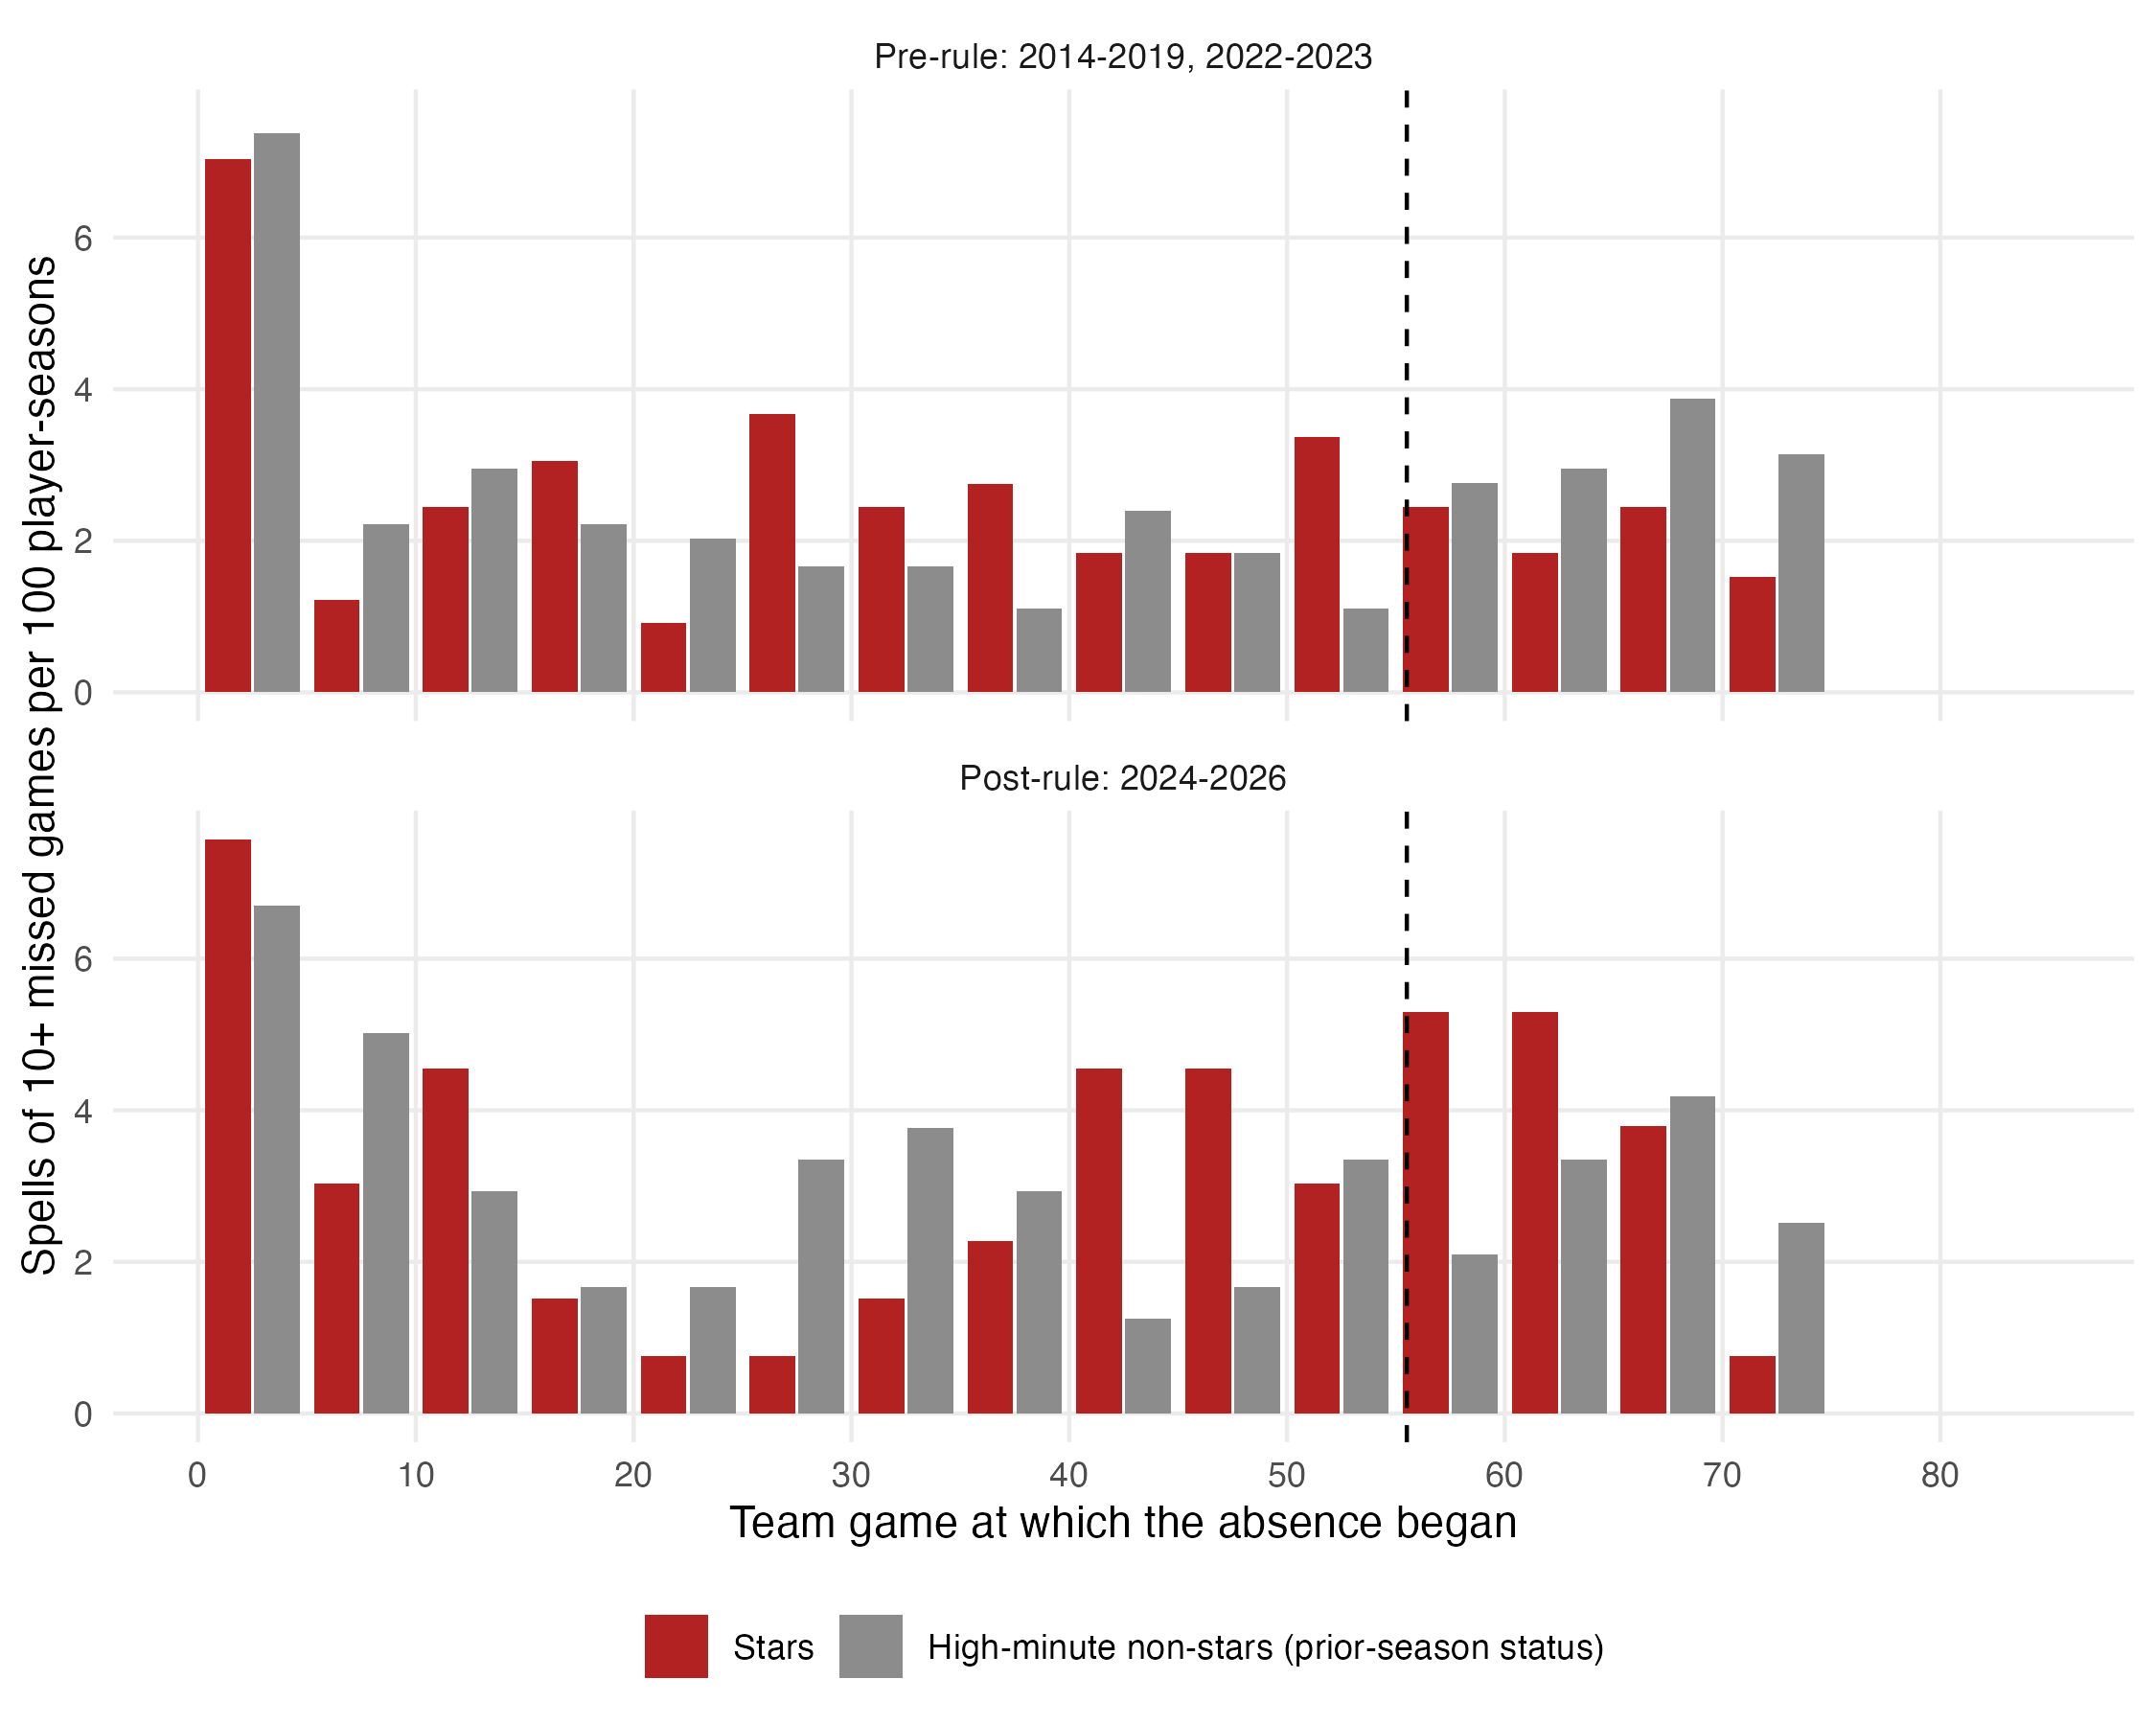
\includegraphics[width=\linewidth]{../../results/figures/paper/figA2_absence_timing.png}
\caption{Team game at which spells of 10 or more missed games began, per 100 player-seasons, stars and control, before and after the rule.}
\label{fig:figA2_absence_timing}
\end{figure}

\begin{figure}[p]
\centering
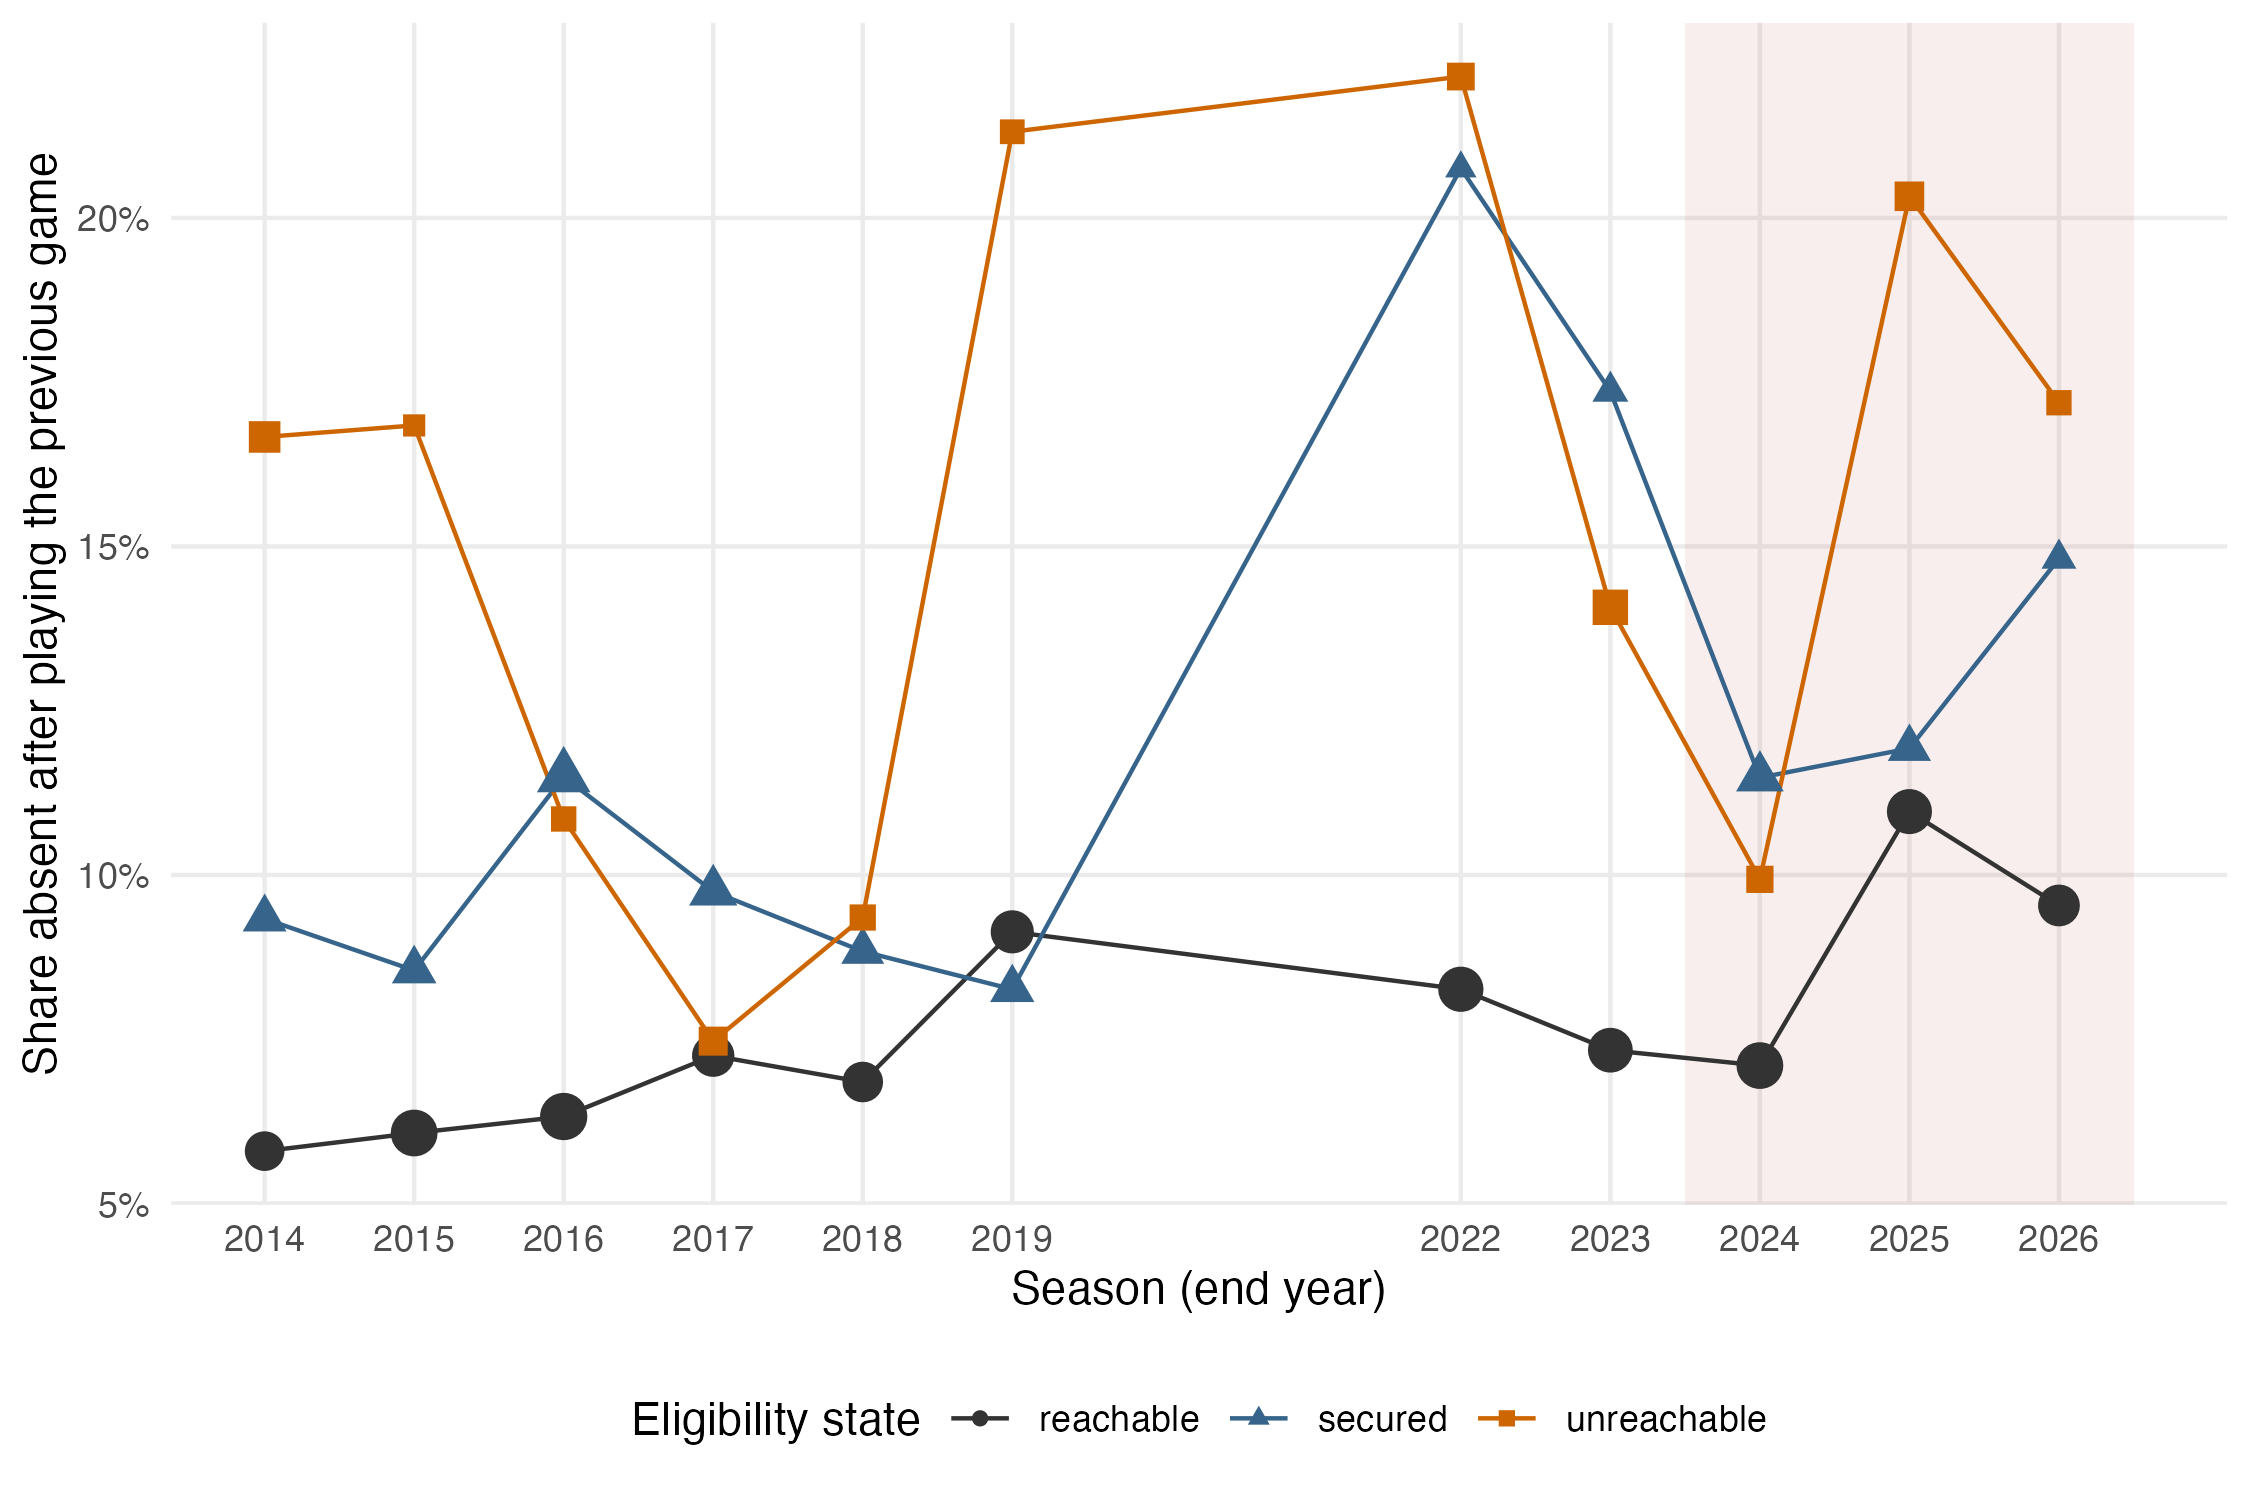
\includegraphics[width=\linewidth]{../../results/figures/paper/figA3_absence_by_state_by_season.png}
\caption{Late-season absence of stars who played the previous game, by eligibility state and season; point size is the number of player-games in the cell.}
\label{fig:figA3_absence_by_state_by_season}
\end{figure}

\clearpage
\section*{Appendix tables}
\begin{table}[!h]
\centering
\caption{\label{tab:tabA1_absence_event_study}Star minus non-star late-season absence by season}
\centering
\resizebox{\ifdim\width>\linewidth\linewidth\else\width\fi}{!}{
\begin{threeparttable}
\begin{tabular}[t]{rllllll}
\toprule
Season & Full, ref 2023: est (SE) & MDE & Full, ref 2017: est (SE) & MDE  & ESPN rows only, ref 2023: est (SE) & MDE  \\
\midrule
2014 & NA & NA & NA & NA & 0.023 (0.014) & 0.038\\
2015 & 0.010 (0.020) & 0.057 & 0.008 (0.019) & 0.054 & 0.009 (0.014) & 0.040\\
2016 & 0.001 (0.022) & 0.062 & -0.002 (0.021) & 0.058 & 0.023 (0.015) & 0.041\\
2017 & 0.006 (0.018) & 0.049 & 0.000 (0.000) & 0.000 & 0.018 (0.012) & 0.034\\
2018 & 0.005 (0.020) & 0.056 & 0.003 (0.019) & 0.053 & -0.002 (0.011) & 0.032\\
2019 & 0.035 (0.022) & 0.062 & 0.033 (0.022) & 0.061 & -0.001 (0.015) & 0.043\\
2022 & 0.031 (0.020) & 0.057 & 0.029 (0.021) & 0.060 & 0.012 (0.013) & 0.036\\
2023 & 0.000 (0.000) & 0.000 & -0.008 (0.021) & 0.059 & 0.000 (0.000) & 0.000\\
2024 & -0.008 (0.018) & 0.050 & -0.010 (0.020) & 0.055 & -0.009 (0.008) & 0.023\\
2025 & -0.017 (0.025) & 0.069 & -0.019 (0.026) & 0.074 & -0.005 (0.014) & 0.039\\
2026 & -0.018 (0.024) & 0.068 & -0.020 (0.025) & 0.071 & -0.021 (0.010) & 0.029\\
\bottomrule
\end{tabular}
\begin{tablenotes}
\item \textit{Note: } 
\item Coefficients on star x season; player, season and team-game-number fixed effects; SEs clustered by player. 'ESPN rows only' reproduces the exploratory construction in which only games with an ESPN row enter.
\end{tablenotes}
\end{threeparttable}}
\end{table}


\begin{table}[!h]
\centering
\caption{\label{tab:tabA2_minute_bins}Minutes played by late-season stars, by slack: share of player-games (cell count)}
\centering
\resizebox{\ifdim\width>\linewidth\linewidth\else\width\fi}{!}{
\begin{threeparttable}
\begin{tabular}[t]{llllll}
\toprule
Sample & Minutes & pre, not tight & pre, tight & post, not tight & post, tight\\
\midrule
All & <15 & 0.018 (103) & 0.010 (7) & 0.007 (16) & 0.000 (0)\\
All & 15-19 & 0.030 (173) & 0.031 (22) & 0.010 (22) & 0.011 (2)\\
All & 20-22 & 0.037 (211) & 0.042 (30) & 0.026 (57) & 0.043 (8)\\
All & 23-30 & 0.243 (1385) & 0.294 (209) & 0.215 (470) & 0.368 (68)\\
All & 31+ & 0.671 (3823) & 0.623 (442) & 0.742 (1622) & 0.578 (107)\\
Played each of previous 3 games & <15 & 0.013 (58) & 0.013 (7) & 0.004 (7) & 0.000 (0)\\
Played each of previous 3 games & 15-19 & 0.021 (98) & 0.033 (17) & 0.009 (15) & 0.000 (0)\\
Played each of previous 3 games & 20-22 & 0.031 (142) & 0.034 (18) & 0.026 (43) & 0.034 (4)\\
Played each of previous 3 games & 23-30 & 0.239 (1090) & 0.295 (154) & 0.202 (340) & 0.325 (38)\\
Played each of previous 3 games & 31+ & 0.696 (3176) & 0.625 (326) & 0.759 (1275) & 0.641 (75)\\
\bottomrule
\end{tabular}
\begin{tablenotes}
\item \textit{Note: } 
\item Stars who played, games 56 onward, 2020-2021 excluded. Tight: 0-3 games of slack and 65 not yet secured. Cell counts in parentheses. Confounded by minute restrictions on players returning from injury.
\end{tablenotes}
\end{threeparttable}}
\end{table}


\begin{table}[!h]
\centering
\caption{\label{tab:tabA3_long_absences}Spells of 10 or more consecutive missed games, stars and high-minute non-stars}
\centering
\resizebox{\ifdim\width>\linewidth\linewidth\else\width\fi}{!}{
\begin{threeparttable}
\begin{tabular}[t]{llrrllllllllllll}
\toprule
Group & Period & Player-seasons & Spells & Spells per star-season & Star-seasons with a spell & Mean length & Games lost per star-season & Censored at season end & Reason: injury/illness & Reason: no row & Reason: rest or coach & Begin games 1-20 & 21-40 & 41-55 & 56-82\\
\midrule
Stars & Pre-rule & 327 & 127 & 0.39 & 33\% & 25.6 & 10.0 & 31\% & 30\% & 56\% & 11\% & 35\% & 25\% & 18\% & 21\%\\
Stars & Post-rule & 132 & 65 & 0.49 & 39\% & 22.2 & 11.0 & 34\% & 20\% & 77\% & 0\% & 34\% & 11\% & 25\% & 31\%\\
High-minute non-stars (prior season) & Pre-rule & 542 & 213 & 0.39 & 34\% & 24.0 & 9.4 & 39\% & 32\% & 54\% & 12\% & 38\% & 16\% & 14\% & 32\%\\
High-minute non-stars (prior season) & Post-rule & 239 & 111 & 0.46 & 38\% & 19.9 & 9.2 & 32\% & 32\% & 62\% & 3\% & 35\% & 25\% & 14\% & 26\%\\
\bottomrule
\end{tabular}
\begin{tablenotes}
\item \textit{Note: } 
\item Full team schedule, 2020-2021 excluded. Reason taken from the first game in the spell for which ESPN printed a row; 'no row' spells have no ESPN row at any point.
\end{tablenotes}
\end{threeparttable}}
\end{table}


\begin{table}[!h]
\centering
\caption{\label{tab:tabA4_absence_reasons}What ESPN says about late-season absences of stars who played the previous game}
\centering
\resizebox{\ifdim\width>\linewidth\linewidth\else\width\fi}{!}{
\begin{threeparttable}
\begin{tabular}[t]{llrl}
\toprule
Period & Class & n & Share\\
\midrule
Pre-rule & no row (reason unknown) & 345 & 54.9\%\\
Pre-rule & injury or illness & 113 & 18.0\%\\
Pre-rule & coach's decision & 107 & 17.0\%\\
Pre-rule & rest & 52 & 8.3\%\\
Pre-rule & other & 11 & 1.8\%\\
Post-rule & no row (reason unknown) & 221 & 81.0\%\\
Post-rule & injury or illness & 41 & 15.0\%\\
Post-rule & rest & 7 & 2.6\%\\
Post-rule & other & 4 & 1.5\%\\
\bottomrule
\end{tabular}
\begin{tablenotes}
\item \textit{Note: } 
\item Classes from the DNP reason string. Absences with no ESPN row carry no reason.
\end{tablenotes}
\end{threeparttable}}
\end{table}


\begin{table}[!h]
\centering
\caption{\label{tab:tabA5_bbr_validation}Games played: ten star-seasons checked against Basketball-Reference}
\centering
\resizebox{\ifdim\width>\linewidth\linewidth\else\width\fi}{!}{
\begin{threeparttable}
\begin{tabular}[t]{rlrllllll}
\toprule
Season & Player & Reference games played & This paper: regular season & Raw ESPN count & Games under the rule (incl. Cup final) & Qualifying games & Status & Source\\
\midrule
2024 & Joel Embiid & 39 & 39 & 39 & 39 & 39 & match & web lookup 2026-09-15 (ESPN game log, StatMuse); BBR not re-requested\\
2024 & Tyrese Haliburton & 69 & 69 & 71 & 70 & 69 & match & cached BBR awards\_2024.html (MIP and All-NBA voting tables, G column)\\
2023 & Stephen Curry & 56 & 56 & 56 & 56 & 56 & match & cached BBR awards\_2023.html (MVP voting table, G column)\\
2025 & Luka Doncic & 50 & 50 & 50 & 50 & 50 & match & web lookup 2026-09-15 (22 DAL + 28 LAL); BBR not re-requested\\
2024 & Nikola Jokic & 79 & 79 & 80 & 79 & 79 & match & cached BBR awards\_2024.html (MVP voting table, G column)\\
2023 & LeBron James & 55 & 55 & 56 & 55 & 55 & match & cached BBR awards\_2023.html (All-NBA voting table, G column)\\
2022 & Kawhi Leonard & 0 &  &  &  &  & no ESPN rows; not in sample & missed the entire 2021-22 season (ACL); web lookup 2026-09-15\\
2024 & Jimmy Butler & 60 & 60 & 60 & 60 & 60 & match & web lookup 2026-09-15; BBR not re-requested\\
2024 & Donovan Mitchell & 55 & 55 & 56 & 55 & 55 & match & web lookup 2026-09-15 (StatMuse); BBR not re-requested\\
2026 & Victor Wembanyama & 64 & 64 & 67 & 65 & 65 & match & cached BBR awards\_2026.html (MVP, DPOY, All-NBA voting tables, G column)\\
\bottomrule
\end{tabular}
\begin{tablenotes}
\item \textit{Note: } 
\item Reference values from cached Basketball-Reference award-voting tables where available, otherwise from a web lookup on the date shown. Regular-season games exclude the All-Star game and the NBA Cup final, as Basketball-Reference does; the rule's count includes the Cup final.
\end{tablenotes}
\end{threeparttable}}
\end{table}


\begin{table}[!h]
\centering
\caption{\label{tab:tabA6_stars_no_appearance}Flagged stars absent from the sample: no ESPN box-score row in the season}
\centering
\resizebox{\ifdim\width>\linewidth\linewidth\else\width\fi}{!}{
\begin{threeparttable}
\begin{tabular}[t]{rl}
\toprule
Season & Flagged stars with no ESPN appearance\\
\midrule
2015 & Andrew Bynum\\
2017 & Chris Bosh; Kobe Bryant; Tim Duncan\\
2018 & Chris Bosh; Kobe Bryant; Tim Duncan\\
2019 & Kobe Bryant\\
2020 & Dirk Nowitzki; Dwyane Wade; John Wall; Kevin Durant; Klay Thompson\\
2021 & Dirk Nowitzki; Dwyane Wade; Klay Thompson\\
2022 & Dirk Nowitzki; Dwyane Wade; Kawhi Leonard; Zion Williamson\\
2026 & Kyrie Irving; Tyrese Haliburton\\
\bottomrule
\end{tabular}
\begin{tablenotes}
\item \textit{Note: } 
\item Retired players and players who missed the entire season. They do not enter any player-season count.
\end{tablenotes}
\end{threeparttable}}
\end{table}


\begin{table}[!h]
\centering
\caption{\label{tab:tabA7_exhibition_correction}Effect of removing All-Star and Rising Stars rows on star counts}
\centering
\resizebox{\ifdim\width>\linewidth\linewidth\else\width\fi}{!}{
\begin{threeparttable}
\begin{tabular}[t]{rrrrllllr}
\toprule
Season & Stars & GP changed & QG changed & Mean GP, raw & Mean GP, clean & Mean QG, raw & Mean QG, clean & Crossed 65 only via exhibition\\
\midrule
2014 & 41 & 18 & 10 & 60.7 & 60.3 & 58.2 & 57.9 & 0\\
2015 & 43 & 16 & 11 & 63.5 & 63.2 & 61.1 & 60.9 & 0\\
2016 & 46 & 20 & 16 & 69.5 & 69.1 & 66.4 & 66.0 & 0\\
2017 & 40 & 21 & 17 & 70.8 & 70.2 & 66.7 & 66.3 & 0\\
2018 & 36 & 18 & 15 & 64.7 & 64.2 & 62.6 & 62.2 & 0\\
2019 & 37 & 19 & 13 & 63.6 & 63.1 & 61.9 & 61.6 & 1\\
2022 & 39 & 15 & 10 & 58.5 & 58.1 & 56.9 & 56.7 & 0\\
2023 & 45 & 16 & 14 & 59.7 & 59.4 & 58.8 & 58.4 & 1\\
2024 & 46 & 19 & 14 & 65.5 & 65.0 & 64.8 & 64.5 & 0\\
2025 & 46 & 16 & 0 & 63.1 & 62.4 & 62.0 & 62.0 & 0\\
2026 & 40 & 18 & 0 & 56.1 & 54.8 & 54.4 & 54.4 & 0\\
\bottomrule
\end{tabular}
\begin{tablenotes}
\item \textit{Note: } 
\item Games played also exclude the NBA Cup final (a non-regular-season game for statistics); qualifying games include it, as the rule does.
\end{tablenotes}
\end{threeparttable}}
\end{table}


\begin{table}[!h]
\centering
\caption{\label{tab:tabA8_composition_2024}Decomposition of the 2023 to 2024 change in mean games: stayers, entrants and leavers}
\centering
\resizebox{\ifdim\width>\linewidth\linewidth\else\width\fi}{!}{
\begin{threeparttable}
\begin{tabular}[t]{llllrlllll}
\toprule
Outcome & Mean 2023 (n) & Mean 2024 (n) & Raw change & Stayers: n & Stayers 2023 & Stayers 2024 & Stayers change & Entrants 2024 (n) & Leavers 2023 (n)\\
\midrule
Stars: games played & 59.4 (45) & 65.0 (46) & 5.6 & 39 & 61.3 & 64.2 & 2.9 & 69.6 (7) & 46.7 (6)\\
Stars: qualifying games & 58.4 (45) & 64.5 (46) & 6.1 & 39 & 60.6 & 63.7 & 3.0 & 69.3 (7) & 44.2 (6)\\
High-minute non-stars (prior season): games played & 65.6 (82) & 66.1 (90) & 0.6 & 50 & 69.7 & 66.0 & -3.8 & 66.4 (40) & 59.1 (32)\\
\bottomrule
\end{tabular}
\begin{tablenotes}
\item \textit{Note: } 
\item Stayers are players in the group in both seasons; entrants are 2024 members who were not members in 2023; leavers are 2023 members who were not members in 2024. The within-player event-study coefficient is identified from stayers.
\end{tablenotes}
\end{threeparttable}}
\end{table}


\begin{table}[!h]
\centering
\caption{\label{tab:tabA9_cohort_pairs}Fixed-cohort difference-in-differences for each pair of adjacent seasons, games played}
\centering
\resizebox{\ifdim\width>\linewidth\linewidth\else\width\fi}{!}{
\begin{threeparttable}
\begin{tabular}[t]{lrlrllll}
\toprule
Seasons & Stars (n) & Stars: first, second & Controls (n) & Controls: first, second & DiD: est (SE) & p & MDE\\
\midrule
2015->2016 & 42 & 64.7, 67.5 & 85 & 66.3, 65.0 & 4.15 (3.77) & 0.27 & 10.6\\
2016->2017 & 42 & 70.5, 69.0 & 69 & 67.4, 66.2 & -0.31 (3.06) & 0.92 & 8.6\\
2017->2018 & 39 & 70.8, 63.3 & 74 & 66.2, 62.2 & -3.59 (3.89) & 0.36 & 10.9\\
2018->2019 & 36 & 64.2, 63.3 & 72 & 63.9, 63.3 & -0.31 (5.16) & 0.95 & 14.5\\
2022->2023 & 38 & 58.4, 60.1 & 73 & 61.1, 63.7 & -0.92 (3.93) & 0.82 & 11.0\\
2023->2024 & 44 & 60.5, 63.3 & 80 & 65.8, 63.9 & 4.66 (3.44) & 0.18 & 9.6\\
2024->2025 & 46 & 65.0, 63.0 & 86 & 66.9, 61.0 & 3.91 (3.32) & 0.24 & 9.3\\
2025->2026 & 43 & 62.5, 52.9 & 79 & 61.5, 57.0 & -5.16 (4.64) & 0.27 & 13.0\\
\bottomrule
\end{tabular}
\begin{tablenotes}
\item \textit{Note: } 
\item Groups fixed at their status in the first season of the pair; players present in both seasons; player and season fixed effects; SEs clustered by player. The 2023 to 2024 row is the year the rule took effect.
\end{tablenotes}
\end{threeparttable}}
\end{table}


\begin{table}[!h]
\centering
\caption{\label{tab:tabA10_bound_windows}The maximal-effect bound under alternative definitions of the at-risk population}
\centering
\resizebox{\ifdim\width>\linewidth\linewidth\else\width\fi}{!}{
\begin{threeparttable}
\begin{tabular}[t]{rlllllll}
\toprule
Slack measured at game & Window & Period & At risk per season & Share of stars & Did not reach & Bound, minimal crossing & Bound, play every game\\
\midrule
55 & 0-12 & Pre-rule & 16.8 & 0.41 & 6.0 & 1.07 & 2.42\\
55 & 0-12 & Post-rule & 20.7 & 0.47 & 7.3 & 1.71 & 3.79\\
55 & 0-8 & Pre-rule & 9.5 & 0.23 & 4.6 & 0.89 & 1.55\\
55 & 0-8 & Post-rule & 9.7 & 0.22 & 5.3 & 1.30 & 2.10\\
62 & 0-12 & Pre-rule & 17.9 & 0.44 & 5.4 & 0.75 & 2.05\\
62 & 0-12 & Post-rule & 20.3 & 0.46 & 5.7 & 0.99 & 2.55\\
62 & 0-8 & Pre-rule & 10.2 & 0.25 & 4.5 & 0.67 & 1.28\\
62 & 0-8 & Post-rule & 11.3 & 0.26 & 5.3 & 0.98 & 1.83\\
\bottomrule
\end{tabular}
\begin{tablenotes}
\item \textit{Note: } 
\item Same construction as Table 5c with slack measured at team game 62 or 55 and the window widened to 0-12 games.
\end{tablenotes}
\end{threeparttable}}
\end{table}


\begin{table}[!h]
\centering
\caption{\label{tab:tabA11_exact65}Finishing at exactly 65 qualifying games among stars who reached the line}
\centering
\resizebox{\ifdim\width>\linewidth\linewidth\else\width\fi}{!}{
\begin{threeparttable}
\begin{tabular}[t]{llrrlll}
\toprule
Sample & Period & n & Finished at exactly 65 & Share & Mean final qualifying games & Fisher p\\
\midrule
all star reachers & Pre-rule & 192 & 9 & 0.05 & 73.7 & 0.16\\
all star reachers & Post-rule & 75 & 7 & 0.09 & 72.7 & 0.16\\
at-risk reachers & Pre-rule & 46 & 8 & 0.17 & 67.3 & 0.19\\
at-risk reachers & Post-rule & 18 & 6 & 0.33 & 67.8 & 0.19\\
healthy at-risk reachers & Pre-rule & 42 & 8 & 0.19 & 67.1 & 0.27\\
healthy at-risk reachers & Post-rule & 14 & 5 & 0.36 & 67.9 & 0.27\\
\bottomrule
\end{tabular}
\begin{tablenotes}
\item \textit{Note: } 
\item At-risk: 0-8 games of slack at team game 62. Healthy: played at least two of games 60-62. Fisher exact test of pre vs post within sample.
\end{tablenotes}
\end{threeparttable}}
\end{table}


\begin{table}[!h]
\centering
\caption{\label{tab:tabA11b_exact65_distribution}Final qualifying games of at-risk stars who reached 65}
\centering
\resizebox{\ifdim\width>\linewidth\linewidth\else\width\fi}{!}{
\begin{tabular}[t]{lrlrl}
\toprule
Final qualifying games & Pre: n & Pre: share & Post: n & Post: share\\
\midrule
65 & 8 & 0.17 & 6 & 0.33\\
66 & 13 & 0.28 & 0 & 0.00\\
67 & 7 & 0.15 & 2 & 0.11\\
68 & 8 & 0.17 & 3 & 0.17\\
69 & 3 & 0.07 & 1 & 0.06\\
70 & 2 & 0.04 & 4 & 0.22\\
71 & 3 & 0.07 & 1 & 0.06\\
72 & 2 & 0.04 & 1 & 0.06\\
\bottomrule
\end{tabular}}
\end{table}


\begin{table}[!h]
\centering
\caption{\label{tab:tabA12_share20_event_study}Share of appearances lasting at least 20 minutes: stars relative to the control group}
\centering
\resizebox{\ifdim\width>\linewidth\linewidth\else\width\fi}{!}{
\begin{threeparttable}
\begin{tabular}[t]{rlllllll}
\toprule
Season & Stars: share 20+ min & Control: share 20+ min & All games, no player FE: star x season (SE) & All games: star x season (SE) & MDE & Late season: star x season (SE) & MDE \\
\midrule
2015 & 0.946 & 0.906 & -0.027 (0.025) & -0.025 (0.024) & 0.068 & -0.073 (0.032) & 0.089\\
2016 & 0.941 & 0.875 & -0.002 (0.032) & -0.001 (0.020) & 0.056 & -0.031 (0.025) & 0.069\\
2017 & 0.932 & 0.913 & -0.049 (0.034) & 0.001 (0.022) & 0.062 & 0.007 (0.024) & 0.068\\
2018 & 0.960 & 0.916 & -0.024 (0.026) & 0.018 (0.019) & 0.052 & 0.017 (0.024) & 0.068\\
2019 & 0.964 & 0.923 & -0.027 (0.024) & 0.017 (0.019) & 0.053 & -0.002 (0.028) & 0.078\\
2022 & 0.970 & 0.937 & -0.035 (0.024) & -0.013 (0.021) & 0.059 & -0.000 (0.026) & 0.073\\
2024 & 0.985 & 0.903 & 0.015 (0.021) & 0.043 (0.016) & 0.044 & 0.072 (0.024) & 0.067\\
2025 & 0.984 & 0.922 & -0.006 (0.020) & 0.040 (0.013) & 0.035 & 0.057 (0.016) & 0.044\\
2026 & 0.981 & 0.912 & 0.001 (0.024) & 0.055 (0.016) & 0.044 & 0.080 (0.020) & 0.056\\
\bottomrule
\end{tabular}
\begin{tablenotes}
\item \textit{Note: } 
\item Player-games in which the player appeared, stars and lagged high-minute non-stars, 2015-2026 excluding 2020-2021. Coefficients on star x season relative to 2023; player, season and team-game-number fixed effects; SEs clustered by player.
\end{tablenotes}
\end{threeparttable}}
\end{table}


\begin{table}[!h]
\centering
\caption{\label{tab:tabA13_late_onset}Long absences beginning in the late-season window, before and after the rule}
\centering
\resizebox{\ifdim\width>\linewidth\linewidth\else\width\fi}{!}{
\begin{threeparttable}
\begin{tabular}[t]{llrrll}
\toprule
Group & Period & Spells & Beginning at game 56+ & Share & Fisher p (pre vs post)\\
\midrule
Stars & Pre-rule & 127 & 27 & 0.21 & 0.16\\
Stars & Post-rule & 65 & 20 & 0.31 & 0.16\\
High-minute non-stars (prior season) & Pre-rule & 213 & 69 & 0.32 & 0.25\\
High-minute non-stars (prior season) & Post-rule & 111 & 29 & 0.26 & 0.25\\
\bottomrule
\end{tabular}
\begin{tablenotes}
\item \textit{Note: } 
\item Difference in shares, stars minus control, post minus pre: 0.158 with bootstrap 95\% interval [-0.012, 0.329] from 2,000 resamples of spells within group and period.
\end{tablenotes}
\end{threeparttable}}
\end{table}


\begin{table}[!h]
\centering
\caption{\label{tab:tabA14_bbr_boxscore_check}ESPN box-score rows against Basketball-Reference did-not-play and inactive lists, sample games}
\centering
\resizebox{\ifdim\width>\linewidth\linewidth\else\width\fi}{!}{
\begin{threeparttable}
\begin{tabular}[t]{rlrrrrrrrll}
\toprule
Season & Game & ESPN rows & BBR box rows & ESPN rows found in BBR box & ESPN DNP rows & Of which BBR did-not-play & BBR inactive & BBR inactive with an ESPN row & Star with no ESPN row & On BBR inactive list\\
\midrule
2015 & 2014-12-03 & 26 & 68 & 26 & 6 & 6 & 3 & 0 & DeMar DeRozan & TRUE\\
2017 & 2016-12-28 & 26 & 68 & 26 & 7 & 7 & 4 & 0 & Damian Lillard & TRUE\\
2019 & 2018-11-15 & 25 & 67 & 25 & 4 & 4 & 8 & 0 & Pau Gasol & TRUE\\
2023 & 2023-01-31 & 28 & 70 & 28 & 8 & 8 & 6 & 0 & Zion Williamson & TRUE\\
2024 & 2024-01-15 & 25 & 67 & 25 & 7 & 7 & 9 & 0 & Jaylen Brown & TRUE\\
2025 & 2025-03-15 & 25 & 67 & 25 & 3 & 3 & 11 & 0 & Ja Morant & TRUE\\
2026 & 2026-03-07 & 26 & 68 & 26 & 5 & 5 & 10 & 0 & Jaren Jackson Jr. & TRUE\\
\bottomrule
\end{tabular}
\begin{tablenotes}
\item \textit{Note: } 
\item One game per season, chosen so that a star has an ESPN no-row absence. BBR box scores list did-not-play and did-not-dress players inside the box and inactive players below it.
\end{tablenotes}
\end{threeparttable}}
\end{table}


\end{document}
